% !TeX root = RJwrapper.tex

\title{Rfssa: An R Package for Functional Singular Spectrum Analysis}
\author{by Hossein Haghbin, Jordan Trinka and Mehdi Maadooliat}

\maketitle

\begin{abstract}
Functional Singular Spectrum Analysis (FSSA) is a non-parametric approach for analyzing Functional Time Series (FTS) and Multivariate FTS (MFTS) data. This paper introduces Rfssa, an R package that addresses implementing FSSA for FTS and MFTS data types. Rfssa provides a flexible container, the funts class, for FTS/MFTS data observed on one-dimensional or multi-dimensional domains. It accepts arbitrary basis systems and offers powerful graphical tools for visualizing time-varying features and pattern changes. The package incorporates two forecasting algorithms for FTS data. Developed using object-oriented programming and Rcpp/RcppArmadillo, Rfssa ensures computational efficiency. The paper covers theoretical background, technical details, usage examples, and highlights potential applications of Rfssa.\end{abstract}

\section{Introduction}\label{sec:introduction}
In recent times, advancements in data acquisition techniques have made it possible to collect data in high-resolution formats. Due to the presence of temporal-spatial dependence, one may consider this type of data as \textit{functional data}. 
Functional Data Analysis (FDA) focuses on developing statistical methodologies for analyzing data represented as functions or curves. While FDA methods are particularly well-suited for handling smooth continuum data, they can also be adapted and extended to effectively analyze functional data that may not exhibit perfect smoothness, including high-resolution data and data with inherent variability.
The widely-used \proglang{R} package for FDA is \CRANpkg{fda} \citep{fdapackage}, which is designed to support analysis of functional data, as described in the textbook by \cite{ramsay2005}. Additionally, there are over 40 other \proglang{R} packages available on CRAN that incorporate functional data analysis, such as \CRANpkg{funFEM} \citep{funFEMpackage}, \CRANpkg{fda.usc} \citep{fdauscpackage}, \CRANpkg{refund} \citep{refundpackage}, \CRANpkg{fdapace} \citep{fdapacepackage}, \CRANpkg{funData} \citep{funDatapackage}, \CRANpkg{ftsspec} \citep{ftsspecpackage}, \CRANpkg{rainbow} \citep{rainbowpackage}, and \CRANpkg{ftsa} \citep{ftsapackage}.

One crucial initial requirement for any of these packages is to establish a framework for representing and storing infinite-dimensional functional observations. The \CRANpkg{fda} package, for instance, employs the \code{fd} class as a container for functional data defined on a one-dimensional (1D) domain. An \code{fd} object represents functional data as a finite linear combination of known basis functions (e.g., Fourier, B-splines, etc.), storing both the basis functions and their respective coefficients for each curve. This representation aligns with the practical implementation found in many papers within the field of FDA. Conversely, several other \proglang{R} packages store functional data in a discrete form evaluated on grid points (e.g., \CRANpkg{fda.usc}, \CRANpkg{refund}, \CRANpkg{funData}, \CRANpkg{rainbow}, and \CRANpkg{fdapace}). These packages also provide the capability to analyze functions beyond the one-dimensional case, such as image data treated as two-dimensional (2D) functions (e.g., \CRANpkg{refund}, \CRANpkg{fdasrvf}, and \CRANpkg{funData}). To the best of our knowledge, packages that support representation beyond 1D functions utilize the grid point representation for execution and storage.
Moreover, recent packages have been developed to handle multivariate functional data, which consist of more than one function per observation unit. Examples of such packages include \CRANpkg{roahd}, \CRANpkg{fda.usc}, and \CRANpkg{funData}.

While some recent FDA packages have focused on analyzing and implementing techniques for Functional Time Series (FTS), where sequences of functions are observed over time, none of them handle Multivariate FTS (MFTS) or multidimensional MFTS.  For example see the packages \CRANpkg{ftsspec}, \CRANpkg{rainbow} and \CRANpkg{ftsa}. In summary, there is still a need for a unified and flexible container for FTS/MFTS data, defined on either one or multidimensional domains. The \code{funts} class in \CRANpkg{Rfssa} \citep{rfssapackage},
the package discussed in this article, aims to address this gap. One of the primary contributions of the package is its capacity to handle and visualize 2-dimensional FTS, including image data. Furthermore, the package accommodates MFTS, especially when observed on distinct domains. This flexibility empowers users to analyze and visualize FTS with multiple variables, even when they do not share the same domain. Notably, the \CRANpkg{Rfssa} package introduces novel visualization tools (as exemplified in Figure \ref{fig:call_center}). These tools include heatmaps and 3D plots, thoughtfully designed to provide a deeper understanding of functional patterns over time. They enhance the ability to discern trends and variations that might remain inconspicuous in conventional plots. An additional feature of the \code{funts} class is its ability to accept any arbitrary basis system as input for the class constructor, including fda basis functions or even empirical basis represented as matrices evaluated at grid points. The classes in the \CRANpkg{Rfssa} package are developed using the S3 object-oriented programming system, and for computational efficiency, significant portions of the package are implemented using the \CRANpkg{Rcpp}/\CRANpkg{RcppArmadillo} packages. Notably, the package includes a shiny web application that provides a user-friendly GUI for implementing Functional Singular Spectrum Analysis (FSSA) on real or simulated FTS/MFTS data.

The \CRANpkg{Rfssa} package was initially developed to implement FSSA for FTS, as discussed in the work of \cite{haghbin2021}. FSSA extends Singular Spectrum Analysis (SSA), a model-free procedure commonly used to analyze time series data. The primary goal of SSA is to decompose the original series into a collection of interpretable components, such as slowly varying trends, oscillatory patterns, and structureless noise. Notably, SSA does not rely on restrictive assumptions like stationarity, linearity, or normality \citep{golyandina2013}. 
It's worth noting that SSA finds applications beyond the functional framework, including smoothing and forecasting purposes \citep{hassani2013, deCarvalho2017realtime}. The non-functional version of FSSA, known as SSA, has previously been implemented in the \CRANpkg{Rssa} package \citep{rssapackage} and the \CRANpkg{ASSA} package \citep{ASSApackage}.
The \CRANpkg{Rssa} package provides various visualization tools to facilitate the grouping stage, and the \CRANpkg{Rfssa} package includes equivalent functional versions of those tools \citep{golyandina2018singular}. While the foundational theory of FSSA was originally designed for univariate FTS, it has since been extended to handle multidimensional FTS data, referred to as Multivariate FSSA (MFSSA) \citep{trinka2022multivariate}. Furthermore, in line with the developments in SSA for forecasting, two distinct algorithms known as Recurrent Forecasting (FSSA R-forecasting) and Vector Forecasting (FSSA V-forecasting) were introduced for FSSA by \cite{trinka2023functional}. Both these forecasting algorithms, along with the capabilities for handling MFSSA, have been seamlessly integrated into the most recent version of the \CRANpkg{Rfssa} package. 

The remainder of this manuscript is organized as follows. Section 2 introduces the FTS/MFTS data preparation theory used in the \code{funts} class. Section 3 discusses the FSSA methodology, including the basic schema of FSSA, FSSA R-forecasting, and FSSA V-forecasting. Technical details of the \CRANpkg{Rfssa} package are provided in Section 4, where we describe the available classes in the package and illustrate their practical usage with examples of real data. Section 5 focuses on the reconstruction stage and FSSA/MFSSA forecasting. In Section 6, we provide a summary of the embedded shiny app. Finally, we conclude the paper in Section 7.


\section{Data preparation in FTS}\label{sec:preparation}
Define $\textbf{y}_N=(y_1,\ldots,y_N)$ to be a collection of observations from an FTS. In the theory of FTS, $y_i$'s are considered as functions in the space $\mathbb{H}=L^2(\mathcal{T})$ where $\mathcal{T}$ is a compact subset of $\mathbb{R}.$ Let $s\in\mathcal{T}$ and consider $y_i(s)\in\mathbb{R}^p$, the sequence of $\textbf{y}_N$ is called (univariate) FTS if $p=1$, and multivariate FTS (or MFTS) if $p>1.$ 
In the realm of functional data analysis, we operate under the assumption that the underlying sample functions, denoted as $y_{i}(\cdot)$, exhibit smoothness for each sample $i$, where $i=1, \ldots, N$. Nevertheless, in practical scenarios, observations are typically acquired discretely at a set of grid points and are susceptible to contamination by random noise. This phenomenon can be represented as follows:
\begin{equation}\label{discr_data}
	Y_{i,k} = y_{i}(t_k) +\varepsilon_{i,k}, \quad k=1,\ldots, K.
\end{equation}
In this expression, $t_k\in\mathcal{T}$, and $K$ denotes the count of discrete grid points across all samples. The $\varepsilon_{i,k}$ terms represent i.i.d random noises.
To preprocess the raw data, it is customary to employ smoothing techniques, converting the discrete observations $Y_{i,k}$ into a continuous form, $y_{i}(\cdot)$. This is typically performed individually for each variable and sample. One widely used approach is finite basis function expansion \citep{ramsay2005}. In this method, a set of basis functions $\left\lbrace \nu_i \right\rbrace_{ i\in\mathbb{N}}$ is considered (not necessarily orthogonal) for the function space $\mathbb{H}$. Each sample function $y_{i}(\cdot)$ in \eqref{discr_data} is then considered as a finite linear combination of the first $d$ basis functions:
\begin{equation}\label{basis_expan}
	y_i(s)= \sum_{j=1}^d c_{ij}\nu_j(s).
\end{equation}
Subsequently, the coefficients $c_{ij}$ can be estimated using least square techniques. By adopting the linear representation form for the functional data in \eqref{basis_expan}, we establish a correspondence between each function $y_i(\cdot)$ and its coefficient vector ${\pmb c}_i=(c_{ij})_{j=1}^d.$ As a result, the coefficient vectors ${\pmb c}_i$ can serve to store and retrieve the original functions, $y_i(\cdot)$'s. This arises from the inherent isomorphism between two finite vector spaces of the same dimension (in this case, $d$). Consequently, ${\pmb c}_i$'s are stored as the primary attribute of \code{funts} objects within the \CRANpkg{Rfssa} package.
Take  two elements $x, y\in \mathbb{H}$ with corresponding coefficient vectors ${\pmb c}_x$ and ${\pmb c}_y.$ Then, the inner product of $x, y$ can be computed in matrix form as $\langle x,y \rangle={\pmb c}_x^\top \mathbf{G} {\pmb c}_y$, where $\mathbf{G}=[ \langle \nu_i,\nu_j \rangle ]_{i,j=1}^{d}$ is the Gram matrix.
It is important to note that $\mathbf{G}$ is Hermitian. Furthermore, because the basis functions $\{\nu_i\}_{i=1}^d$ are linearly independent, $\mathbf{G}$ is positive definite, making it invertible \citep[][Thm. 7.2.10]{horn2012matrix}.
Moreover, let $A:\mathbb{H}\rightarrow \mathbb{H}$ be a linear operator and $y=A(x).$ Then, ${\pmb c}_y= \mathbf{G}^{-1}\mathbf{A}{\pmb c}_x,$ where $\mathbf{A}=[ \langle A(\nu_j),\nu_i \rangle ]_{i,j=1}^{d}$ is called the corresponding matrix of the operator $A.$ 

It is worth noting that while the FSSA theory extends to arbitrary dimensions, practical implementation for dimensions greater than $2$ introduces considerable computational complexity. Moreover, high-dimensional FTS data are relatively rare in real-world applications. Therefore, within the \CRANpkg{Rfssa} package, we have chosen to confine the \code{funts} object to support functions observed over domains that are one or two-dimensional. In the \CRANpkg{Rfssa} package, the task of preprocessing the raw discrete observations and converting those to the \code{funts} object is assigned to the \code{funts($\cdot$)} constructor. 

\section{An overview of the FSSA methodology}\label{sec:methodology}
FSSA is a nonparametric technique to decompose FTS and MFTS and the methodology can also be used to forecast such data \citep{haghbin2021, trinka2022multivariate, trinka2023functional}; it can also be used as a visualization tool to illustrate the concept of seasonality and periodicity in the functional space over time.

\subsection{Basic schema of FSSA}
 Basic FSSA consists of two stages where each stage includes two steps. We outline the four steps of the FSSA algorithm here.
\begin{itemize}
\item[I)] \textbf{First stage: decomposition}
\begin{itemize}
\item[1.]  \textit{Embedding} \\ For a positive integer, $L<N/2$, let $\mathbb{H}^L$ be the Cartesian product of $L$ copies of $\mathbb{H}$ and define  the \textit{trajectory} operator $\mathbfcal{X}:\mathbb{R}^{K} \rightarrow \mathbb{H}^{L}$ with
	\begin{equation}\label{trajectory}
		\mathbfcal{X}{\pmb a}:=\sum_{j=1}^K a_j{\pmb x}_j,\qquad
		\ {\pmb a}=\left(a_1,\ldots, a_K\right)^\top \in\mathbb{R}^K.
	\end{equation}
	
	where $K=N-L+1$ and 
	\begin{equation}\label{flvec}
		{\pmb x}_j(s):= \left( y_j(s), y_{j+1}(s), \ldots, y_{j+L-1}(s)\right)^\top,\ j=1,\ldots, K,
	\end{equation}
	are called \textit{lag-vectors}. One may consider the trajectory operator $\mathbfcal{X}$ in \eqref{trajectory} as an $L \times K$ matrix with functional entries in the form of	
	\begin{equation}\label{eqn:hankelmat}
		\mathbfcal{X}(s) = \begin{bmatrix}y_{1}(s) & y_{2}(s) & y_{3}(s) & \cdots & y_{K}(s) \\ y_{2}(s) & y_{3}(s) & y_{4}(s) & \cdots & y_{K+1}(s) \\ y_{3}(s) & y_{4}(s) & y_{5}(s) & \cdots & y_{K+2}(s) \\ \vdots  & \vdots & \vdots & \ddots & \vdots \\ y_{L}(s) & y_{L+1}(s) & y_{L+2}(s) & \cdots & y_{N}(s)  \end{bmatrix}.
	\end{equation}
	
Note that the antidiagonal elements of the matrix in \eqref{eqn:hankelmat} are all equal. Such matrices are called Hankel, and since $\mathbfcal{X}(s)$ is a Hankel matrix for any $s$ in the domain, we call $\mathbfcal{X}$ a Hankel operator. In practice, a main challenge is how to use the original basis of $\mathbb{H}$ to represent the lag-vectors in $\mathbb{H}^L$. To do this, one may define a quotient sequence $q_k$, and a reminder sequence $r_k$, by $k=(q_k-1)L+r_k,$ where $1\leq r_k\leq L$, and $1\leq q_k\leq d$. Now, consider ${\pmb \phi}_{k}$ as a functional vector of length $L$ with all zero functions, except $r_k$-th element, which is $\nu_{q_k}$. Using this definition, the lag-vector ${\pmb{x}_j}$ given in \eqref{flvec} can be represented as a linear combination of $\{{\pmb \phi}_{k}\}_{k=1}^{Ld}$ with the corresponding coefficient vector ${\bf b}_j=(c_{1j},\ldots, c_{1,j+L-1},c_{2j},\ldots,c_{2,j+L-1},\ldots,c_{d,j+L-1} )^\top.$ 
	
\item[2.] \textit{FSVD }\\ We apply the functional singular value decomposition (FSVD) to $\mathbfcal{X}$ and obtain a collection of singular values, $\{\sqrt{\lambda_i}\}_{i=1}^{r}$, orthonormal right singular vectors $\{\mathbf{v}_{i}\}_{i=1}^{r}$ (that are elements of $\mathbb{R}^{K}$), and orthonormal left singular functions $\{\pmb{\psi}_{i}\}_{i=1}^{r}$ (that are elements of $\mathbb{H}^{L}$). The collection $(\sqrt{\lambda_i}, \pmb{\psi}_i, \mathbf{v}_i)$ will be called the $i^{th}$ eigentriple of the FSVD, and $r$ is the rank of $\mathbfcal{X}$:	
	\begin{equation}\label{FSVD}
		\mathbfcal{X} = \sum_{i=1}^{r} \mathbfcal{X}_{i} = \sum_{i=1}^{r} \sqrt{\lambda_i} \mathbf{v}_{i} \otimes \pmb{\psi}_{i},
	\end{equation}
where $\mathbfcal{X}_{i}:\mathbb{R}^{K} \rightarrow \mathbb{H}^{L}$ is a rank one elementary operator. To implement the FSVD of $\mathbfcal{X}$ given in \eqref{FSVD}, let ${\bf B}:=[{\bf b}_1,\cdots,{\bf b}_K]$, $\mathbf{G}:=[ \langle {\pmb \phi}_{i}, {\pmb \phi}_{j} \rangle_{\mathbb{H}^L}]_{i,j=1}^{Ld}$, $\mathbf{X}:=\mathbf{G}^{1/2}\mathbf{B}$, and $\left(\sqrt{\lambda_i}, \pmb{u}_i, \mathbf{v}_i\right)$'s be the eigentriples of the SVD of the matrix $\mathbf{X}$. It can be shown that $\left(\sqrt{\lambda_i},\pmb{\psi}_i,\mathbf{v}_i \right)$ is the $i^{th}$ eigentriple of the FSVD of $\mathbfcal{X}$, where the left singular function, ${\pmb \psi}_i$, is corresponding to the coefficient vector $\mathbf{G}^{-1/2}{\pmb u}_i$. See \citep{haghbin2021} for more details. 
\end{itemize}
These steps can also be extended to multivariate case, i.e. MFSSA. See \cite{trinka2022multivariate} for more details. In the \CRANpkg{Rfssa} package, the results of the decomposition stage is held in an object from the \code{fssa} class. The constructor, \code{fssa($\cdot$)}, performs the decomposition for both FSSA and MFSSA algorithm and returns an object of class \code{fssa}. Further discussion about the attributes and methods of the \code{fssa} class is given in the technical details section.

\item[II)] \textbf{Second stage: reconstruction}
\begin{itemize}
\item[3.] \textit{Grouping}\\ We partition the set of indices $\{1,\dots,r\}$ into disjoint sets $I_{q}$, where $q \in \{1,\dots, m\}$ and $m\leq r$. From here, we obtain the group $\mathbfcal{X}_{I_{q}}$ by combining the respective elementary operators accordingly:	
	\begin{equation}
		\mathbfcal{X}_{I_{q}} = \sum_{i \in I_{q}} \mathbfcal{X}_{i}. \nonumber
	\end{equation}
Exploratory plots of singular values, right singular vectors, and left singular functions that investigate the different modes of variation extracted in the decomposition stage are used to decide how to form the sets, $I_{q}$, and we discuss such plots in further detail in section five.

\item[4.] \textit{Hankelization }\\ Since each $\mathbfcal{X}_{I_{q}}$ is not necessarily Hankel, we perform diagonal averaging of the entries to Hankelize each operator. From each Hankelized $\mathbfcal{X}_{I_{q}}$, we obtain an FTS, $\mathbf{y}_{N}^{q}$, that describes main characteristics of $\mathbf{y}_{N}$ such as mean, seasonal, trend, and noise behaviors.
\end{itemize}
For the reconstruction stage, the \CRANpkg{Rfssa} package provides the function \code{freconstruct($\cdot$)} which returns a list of objects of class \code{funts} associated to the groups specified by the user. If the supplied input to the \code{fssa($\cdot$)} function is an MFTS, the signal extraction process is almost identical as compared to the univariate case with the exception that now, we have that each element of the time series is a tuple of functions comprised of elements observed over one or two-dimensional domains.% 
\end{itemize}
\begin{figure}[ t!]
	\centering
	\includegraphics[page=3,width=.329\textwidth]{figures/call.pdf}
	\includegraphics[page=4,width=.329\textwidth]{figures/call.pdf}
	\includegraphics[page=5,width=.329\textwidth]{figures/call.pdf}
	\includegraphics[page=6,width=.329\textwidth]{figures/call.pdf}
	\includegraphics[page=7,width=.329\textwidth]{figures/call.pdf}
	\includegraphics[page=8,width=.329\textwidth]{figures/call.pdf}
	\caption{(A): Line plot of \code{Callcenter} data; (B): FTS reconstructed using $I_{\mathfrak{s}} = \{1,\cdots,7\}$; (C): FTS reconstructed by 
	setting $I_{1}=\{1\}$; (D): FTS reconstructed using $I_{2} = \{2,3\}$; (E): FTS reconstructed from $I_{3}=\{4,5\}$; (F): FTS reconstructed from $I_{4}=\{6,7\}$.}
	\label{fig:recon_call}
\end{figure}

As a motivating example, consider the \code{Callcenter} dataset Figure 
\ref{fig:recon_call}(A), which has been previously discussed in 
\cite{maadooliat2015integrating} and is included in the package. This dataset 
records the number of calls received by a call center in 1999. Each functional 
observation corresponds to the square root of the daily call count, and the entire 
FTS represents all the days in 1999. 
When dealing with time series data exhibiting known periodic patterns, it is a common practice in SSA to choose the window length, $L$, as a multiple of this underlying periodicity. This choice ensures that the method effectively extracts the corresponding periodic components \citep{golyandina2001}.
For our illustrative example using the \code{Callcenter} dataset, we specifically opt for a window length of $L=28$. This selection allows us to effectively capture the weekly periodic patterns that inherently exist within this functional time series \citep{haghbin2021}. After applying FSSA, we 
obtain reconstructed FTS representations under 
different grouping considerations, as illustrated in Figures 
\ref{fig:recon_call}(B-F). Particularly noteworthy is the reconstructed FTS obtained 
using the leading 7 eigentriples of the FSVD, as shown in Figure 
\ref{fig:recon_call}(B).
It is important to mention that the selection of groups in FTS is typically guided 
by 
various SSA-type plotting tools, which rely on the similarity in the harmonic 
structure of extracted elementary components. Such SSA-type plots have been 
available for non-functional time series in the \CRANpkg{Rssa} package, and analogous 
tools for the functional case have been developed in \CRANpkg{Rfssa} (Figure 
\ref{fig:call_decomp}). However, it's worth noting that this 
extension presented its own set of challenges, both in theory and implementation. 
Detailed code for generating the reconstructed functions shown in Figure 
\ref{fig:recon_call} can be found in the subsequent sections of this paper.


\begin{figure}[t!]
	\centering
	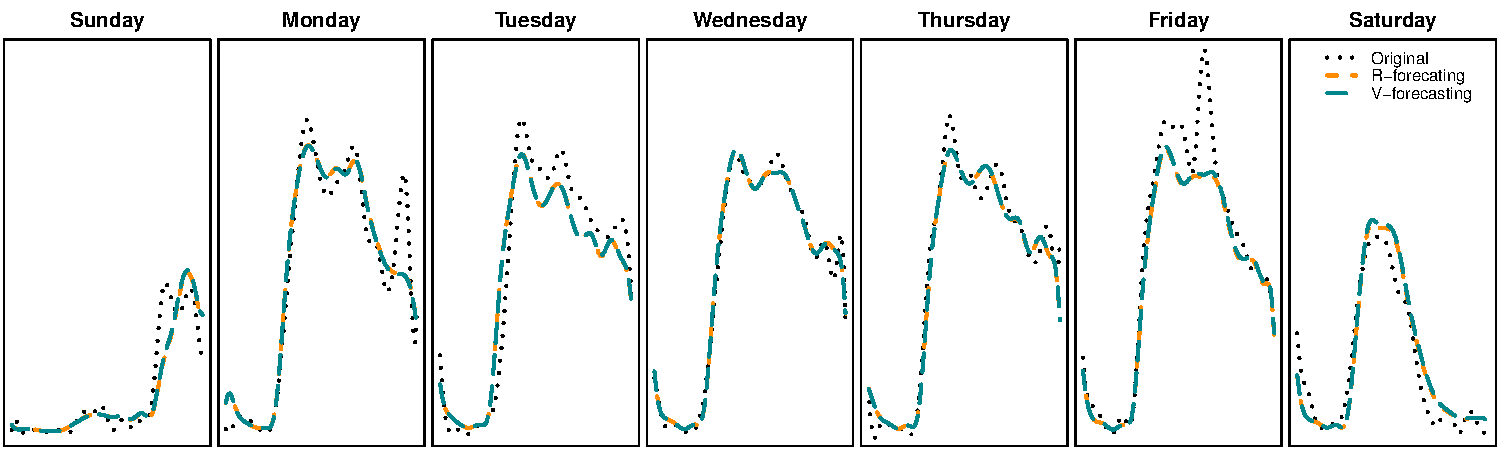
\includegraphics[width=\textwidth]{figures/call_fc.pdf}
	\caption{The prediction of the last 7 days of the year 1999 for the 
		\code{Callcenter} 
		data, based on FSSA R-forecasting and V-forceasting, and comparing the 
		results 
		with the observed functions.}
	\label{fig:for_call}
\end{figure}
\subsection{FSSA Forecasting}\label{subsec:forecast}
After the decomposition stage, one may perform forecasting instead of reconstruction (Figure \ref{fig:roadpap}). R-forecasting and V-forecasting are two main defined approaches in FSSA/MFSSA \citep{trinka2023functional}. In both forecasting methods, the goal is to obtain the FTS, $\mathbf{g}_{N+M}^{q}=\left(g_{1}^{q},\dots,g_{N+M}^{q}\right)$, where the first $N$ terms are close to $\mathbf{y}_{N}^{q}$ and the goal is to forecast the remaining elements, $\{g_{i}^{q}\}_{i=N+1}^{N+M}$.

Forecasts in the R-forecasting method, are obtained using a linear combination of the previous $L-1$ elements of $\mathbf{g}_{N+M}^{q}$. Consider a positive integer $k<r$ and define $\mathbfcal{V} = \sum_{i=1}^{k} \pi_{i} \otimes \pi_{i}$, where $\pi_{i} \in \mathbb{H}$ is the last element of left singular function $\pmb{\psi}_{i}$. Define $\mathbfcal{A}_{j}: \mathbb{H} \rightarrow \mathbb{H}$ such that $\mathbfcal{A}_{j} = \sum_{i=1}^{k}\psi_{j,i} \otimes \left(\mathbfcal{I} - \mathbfcal{V}\right)^{-1}\pi_{i}$, where $\psi_{j,i}$ is the $j^{\text{th}}$ component of $\pmb{\psi}_{i}$, and $\mathbfcal{I}:\mathbb{H} \rightarrow \mathbb{H}$ is the identity operator. Then the R-forecasting can be obtained using following equation
\begin{equation}
	g_{i}^{q}=\begin{cases} 
		y_{i}^{q}, & i=1,\dots,N \\
		\sum_{j=1}^{L-1}\mathbfcal{A}_{j}g_{i+j-L}^{q}, & i=N+1,\dots,N+M.
	\end{cases}
\end{equation}

Forecasts in the V-forecasting method, are obtained by predicting functional vectors. One may define an orthogonal projection, $\pmb{\Pi}:\mathbb{H}^{L-1} \rightarrow \mathbb{H}^{L-1}$, that projects onto the space spanned by $\{\pmb{\psi}_{i}^{\nabla}\}_{i=1}^{k}$, where $\pmb{\psi}_{i}^{\nabla} \in \mathbb{H}^{L-1}$ is formed from the first $L-1$ elements of $\pmb{\psi}_{i}$. Now let $\mathbfcal{Q}:\mathbb{H}^{L} \rightarrow \mathbb{H}^{L}$ be given by 
\begin{equation}
\mathbfcal{Q}\left(\pmb{x}\right)=\begin{pmatrix} \pmb{\Pi}\left(\pmb{x}^{\Delta}\right) \\ \sum_{j=1}^{L-1}\mathbfcal{A}_{j}x^{\Delta}_{j}\end{pmatrix}, \qquad {\pmb{x}} \in \mathbb{H}^{L} \nonumber,
\end{equation}
where $\pmb{x}^{\Delta}$ contains the last $L-1$ components of $\pmb{x}$, and $x_{j}^{\Delta}$ is the $j^{\text{th}}$ component of $\pmb{x}^{\Delta}$. The V-forecasting algorithm is given in the following steps:
\begin{enumerate}
\item[1.] Define $\pmb{w}^{q}_{j}$ as
\[\pmb{w}^{q}_{j}= \begin{cases} 
      \pmb{x}^{q}_{j}, & j=1,\dots, K \\
     \mathbfcal{Q}\pmb{w}^{q}_{j-1}, & j=K+1, \dots, K+M,
   \end{cases}
\]
where $\{\pmb{x}^{q}_{j}\}_{j=1}^{K}$ spans the range of operator $\mathbfcal{X}_{I_{q}}$.
\item[2.] Form the operator $\mathbfcal{W}^q:\mathbb{R}^{K+M} \rightarrow \mathbb{H}^{L}$ whose range is linearly spanned by the set $\{\pmb{w}_{i}^q\}_{i=1}^{K+M}$.
\item[3.] Hankelize $\mathbfcal{W}^q$ in order to extract the FTS $\mathbf{g}^{q}_{N+M}$.
\item[4.] The functions, $g^{q}_{N+1}, \dots, g^{q}_{N+M}$, form the $M$ terms of the FSSA vector forecast.
\end{enumerate}
Continuing from the previous example, we utilized the first 358 days of the year to 
train the FSSA model on the \code{Callcenter} dataset. Subsequently, we employed the 
FSSA R-forecasting and V-forecasting methods to make predictions for the final week 
($len = 7$). Figure \ref{fig:for_call} illustrates both the actual and forecasted 
curves for each day of the week, employing each respective method. Detailed code for 
this process can be found in the subsequent sections.

In the \CRANpkg{Rfssa} package, we offer the \code{fforecast($\cdot$)} function 
designed for the execution of R-forecasting or V-forecasting algorithms. This 
function expects an input argument of class \code{fssa} and yields an output of 
class \code{fforecast}. The latter comprises a list of objects of class 
\code{funts}, with each \code{funts} representing a forecasted group.


\begin{figure}[b!]
	\centering
	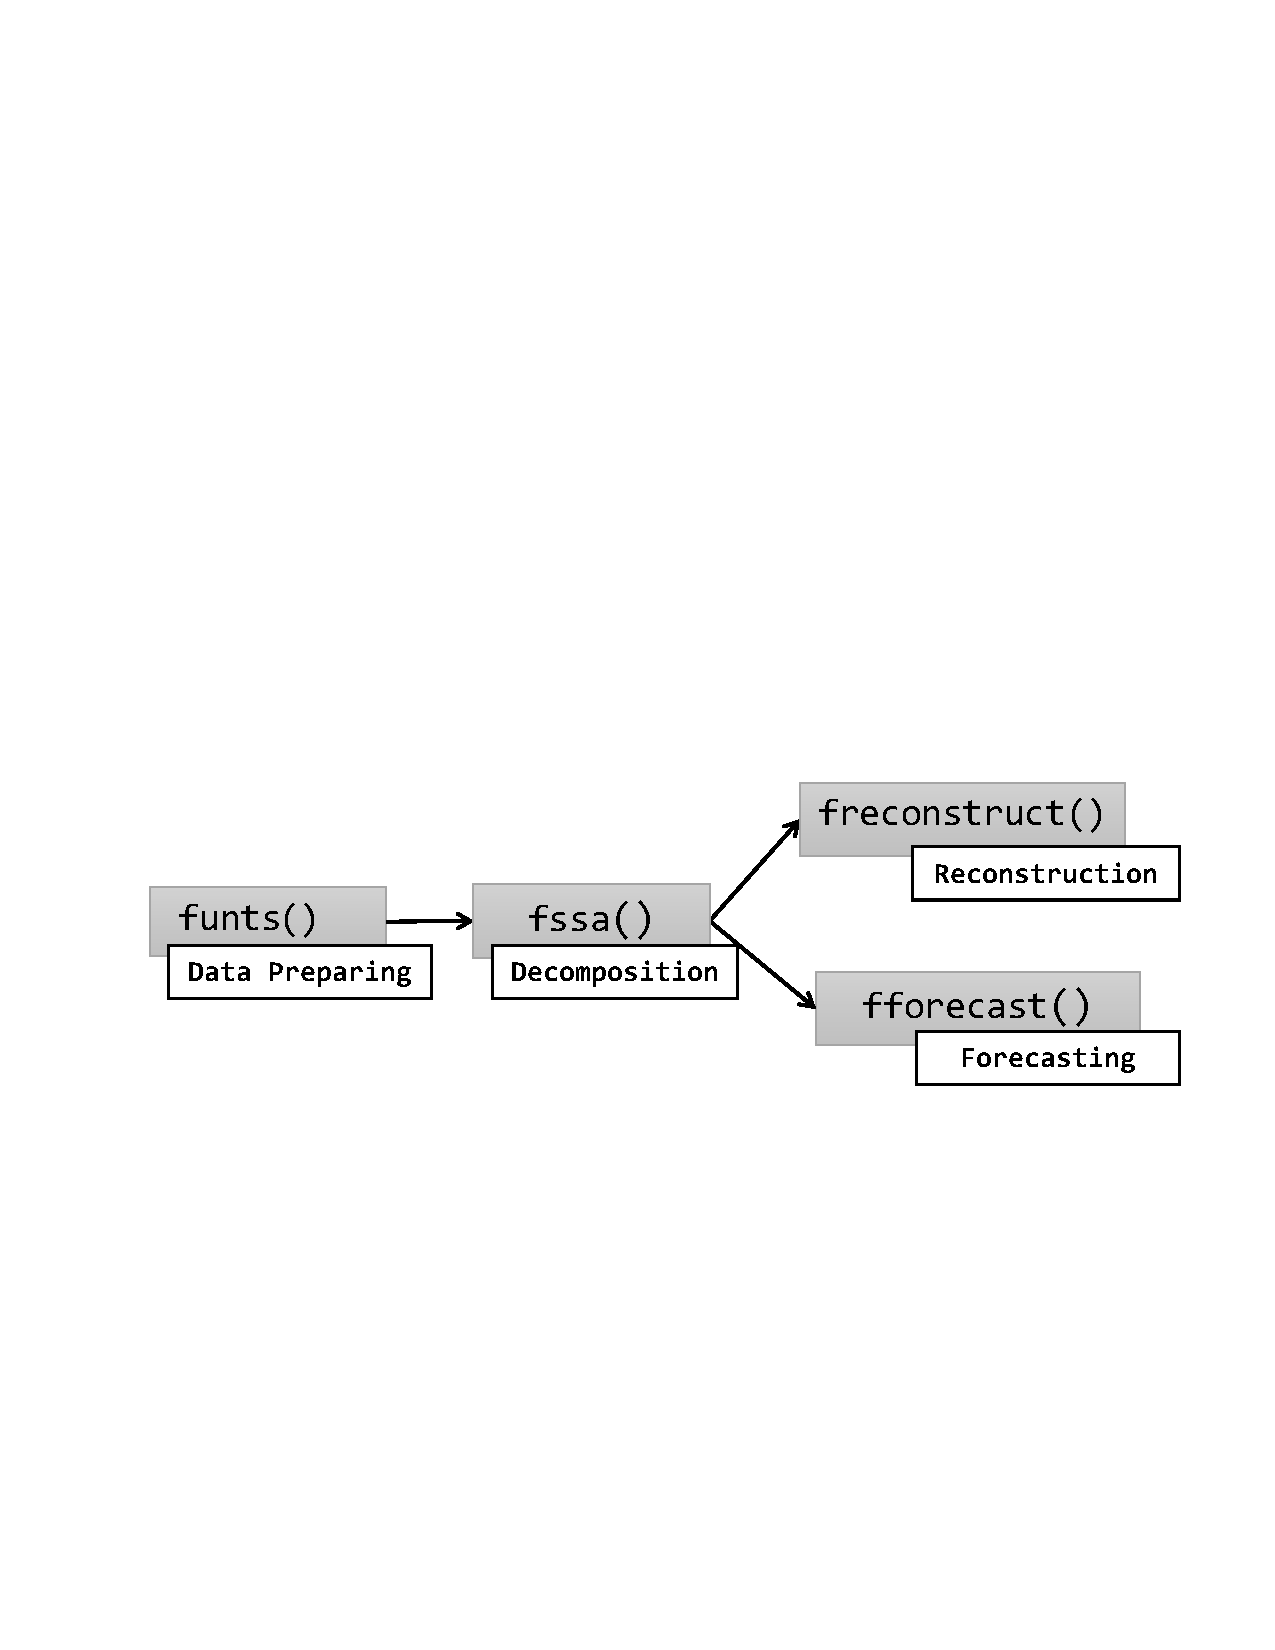
\includegraphics[page=1,width=0.7\textwidth]{figures/roadmap.pdf}
	\caption{The roadmap of the \CRANpkg{Rfssa} package.}
	\label{fig:roadpap}
\end{figure}

\section{Technical details of the Rfssa package}\label{sec:Technical}
The roadmap of the main functions used in the \CRANpkg{Rfssa} package is given in Figure 
\ref{fig:roadpap}. The inputs and outputs of these functions are described in Table 
\ref{tab:1}. As it can be seen from Table \ref{tab:1},  three classes 
(\code{funts}, \code{fssa} and \code{fforecast}) are used to support the return 
objects of theses functions. The \code{funts($\cdot$)}, \code{fssa($\cdot$)} and 
\code{fforecast($\cdot$)} functions are the constructors of the \code{funts}, 
\code{fssa} and \code{fforecast} classes, respectively. In the rest of this 
section we present these classes with illustrative examples, and later we 
describe the reconstruction and forecasting functions in details.

\begin{table}[t!]
	%\centering
	%\small
	\fontsize{9}{12}\selectfont
	\begin{tabular}{ >{\centering}m{2cm} m{3.5 cm} m{4cm} m{3cm}}
		\toprule
		Function & Descriptions & \centering{ Main arguments} & \hspace{1cm}Returns \\ 
		\midrule
		\code{funts($\cdot$)} & Create FTS/MFTS objects   &  Discretely sampled data 
		or coefficients, basis system specifications, a set of argument values 
		corresponding to the observations in X, the time specifications arguments. 
		& An object of class \code{funts}. 
		\\ 
		\midrule
		\code{fssa($\cdot$)} & Performs the decomposition (including embedding and FSVD 
		steps) stage for FTS/MFTS data.& An object of class \code{funts} and window 
		length $L.$ & An object of class \code{fssa}.\\
				\midrule
		\code{freconstruct($\cdot$)} & Performs the reconstruction (including grouping and 
		Hankelization steps) stage.& An object of class \code{fssa} and list of 
		numeric vectors includes indices of elementary components of a group. & A  list of \code{funts} objects reconstructed according to the specified groups.\\
		\midrule
		\code{fforecast($\cdot$)} & Performs FSSA R-forecasting or FSSA V-forecasting.& An 
		object of class \code{fssa}, list of numeric vectors includes indices of 
		elementary components of a group used for reconstruction and forecasting and 
		forecast horizon $h$. & An object of class \code{fforecast}.\\
\bottomrule   
\end{tabular}
\caption{A summary of FSSA written  functions in the \CRANpkg{Rfssa} package.}
\label{tab:1}
\end{table}

\subsection{The \code{funts} class}\label{subsec:fts}
The \code{funts($\cdot$)} constructor is used to create an \code{S3} object of 
class \code{funts}. This object is designed to encapsulate various forms of 
FTS, including both univariate and multivariate types. It offers a 
versatile framework for the creation and manipulation of  \code{funts} objects, 
accommodating different basis systems and dimensions. It accepts 
the following arguments:
 \begin{itemize}
 	\item[-] \code{X}: A matrix, three-dimensional array, or a list of matrix or 
 	array objects. When \code{method="data"}, it represents the observed curve 
 	values at discrete sampling points or argument values. When 
 	\code{method="coefs"}, \code{X} specifies the coefficients corresponding to the 
 	basis system defined in \code{basisobj}. If \code{X} is a list, it defines a 
 	multivariate FTS, with each element being a matrix or three-dimensional array 
 	object. In matrix objects, rows correspond to argument values, and columns 
 	correspond to the length of the FTS. In three-dimensional array objects, the 
 	first and second dimensions correspond to argument values, and the third 
 	dimension to the length of the FTS.	
 	\item[-] \code{basisobj}: This argument should be an object of class 
 	\code{basisfd}, a matrix of empirical basis, or a list of \code{basisfd} or 
 	empirical basis objects. In the case of empirical basis, rows correspond to 
 	basis functions, and columns correspond to grid points.
 	\item[-] \code{argval}: A vector list of length \code{p}, 
 	representing a set of argument values corresponding to the observations in 
 	\code{X}. Each entry in this list should either be a numeric value or a list of 
 	numeric elements, depending on the dimension of the domain over which the 
 	variable is observed. It's worth noting that these values can vary from one 
 	variable to another. If \code{argval} is set to \code{NULL}, the default values 
 	are the integers from 1 to \textit{n}, where \textit{n} is the size of the first 
 	dimension in the \code{X} argument. 	
 	\item[-] \code{method}: This parameter determines the type of the \code{X} 
 	matrix, and it can take one of two values: \code{coefs} or \code{data}. 	
 	\item[-] \code{start} and \code{end}: Specify time of the first and last observations. They can be a 
 	single positive integer or an object of classes \code{Date}, \code{POSIXct}, or 
 	\code{POSIXt}, representing a natural time unit.
 	\item[-] \code{tname}, \code{vnames} and \code{dnames}: These parameters accept strings or lists of strings to specify the names of time, variables, and domains.
 \end{itemize}
The \code{funts($\cdot$)} constructor offers flexibility to users. Users can either provide 
their custom basis or request \CRANpkg{Rfssa} to generate the basis for them, leveraging 
the capabilities of the \CRANpkg{fda} package. It is assumed that each variable is 
observed over a regular and equidistant grid. Furthermore, each variable in the 
\code{funts} object is assumed to be observed over either a one or two-dimensional 
domain, as illustrated in Figure \ref{fig:fts}. 
To enhance the representation of 
time, the \code{funts} function introduces	two parameters, namely \code{start} 
and \code{end}, which capture the time 	series duration. This design allows users to 
specify time information in a	structured and standardized manner. Users have the 
flexibility to set 	\code{start} and \code{end} using various time and date 
classes, such as 	\code{Date}, \code{POSIXct}, or \code{POSIXt}. If users do not 
provide the \code{start} and \code{end} arguments, default values are used, with 
\code{start=1} and \code{end=N}, where $N$ represents the length of the time 
series. This default approach aligns with common practices, as seen in classes 
like \code{ts} in the \CRANpkg{stats} package, as well as \code{fts} classes in 
\CRANpkg{rainbow} or \CRANpkg{ftsa}.
An object of class \code{funts} is a list encompassing the following elements:
	\begin{enumerate}
		\item[-] \code{N}: Represents the length of the time series.
		\item[-] \code{dimSupp}: A list specifying the dimensions of the support 
		domain of 
		the variables.
		\item[-] \code{time}:  The time object.
		\item[-] \code{coefs}:  A list containing basis coefficients.
		\item[-] \code{basis}:  A list of basis systems.
		\item[-] \code{B\_mat}:  Evaluated basis functions on initial arguments.
		\item[-] \code{argval}:  Initial arguments of the observed functions.
	\end{enumerate}

\begin{figure}[ht]
	\centering
	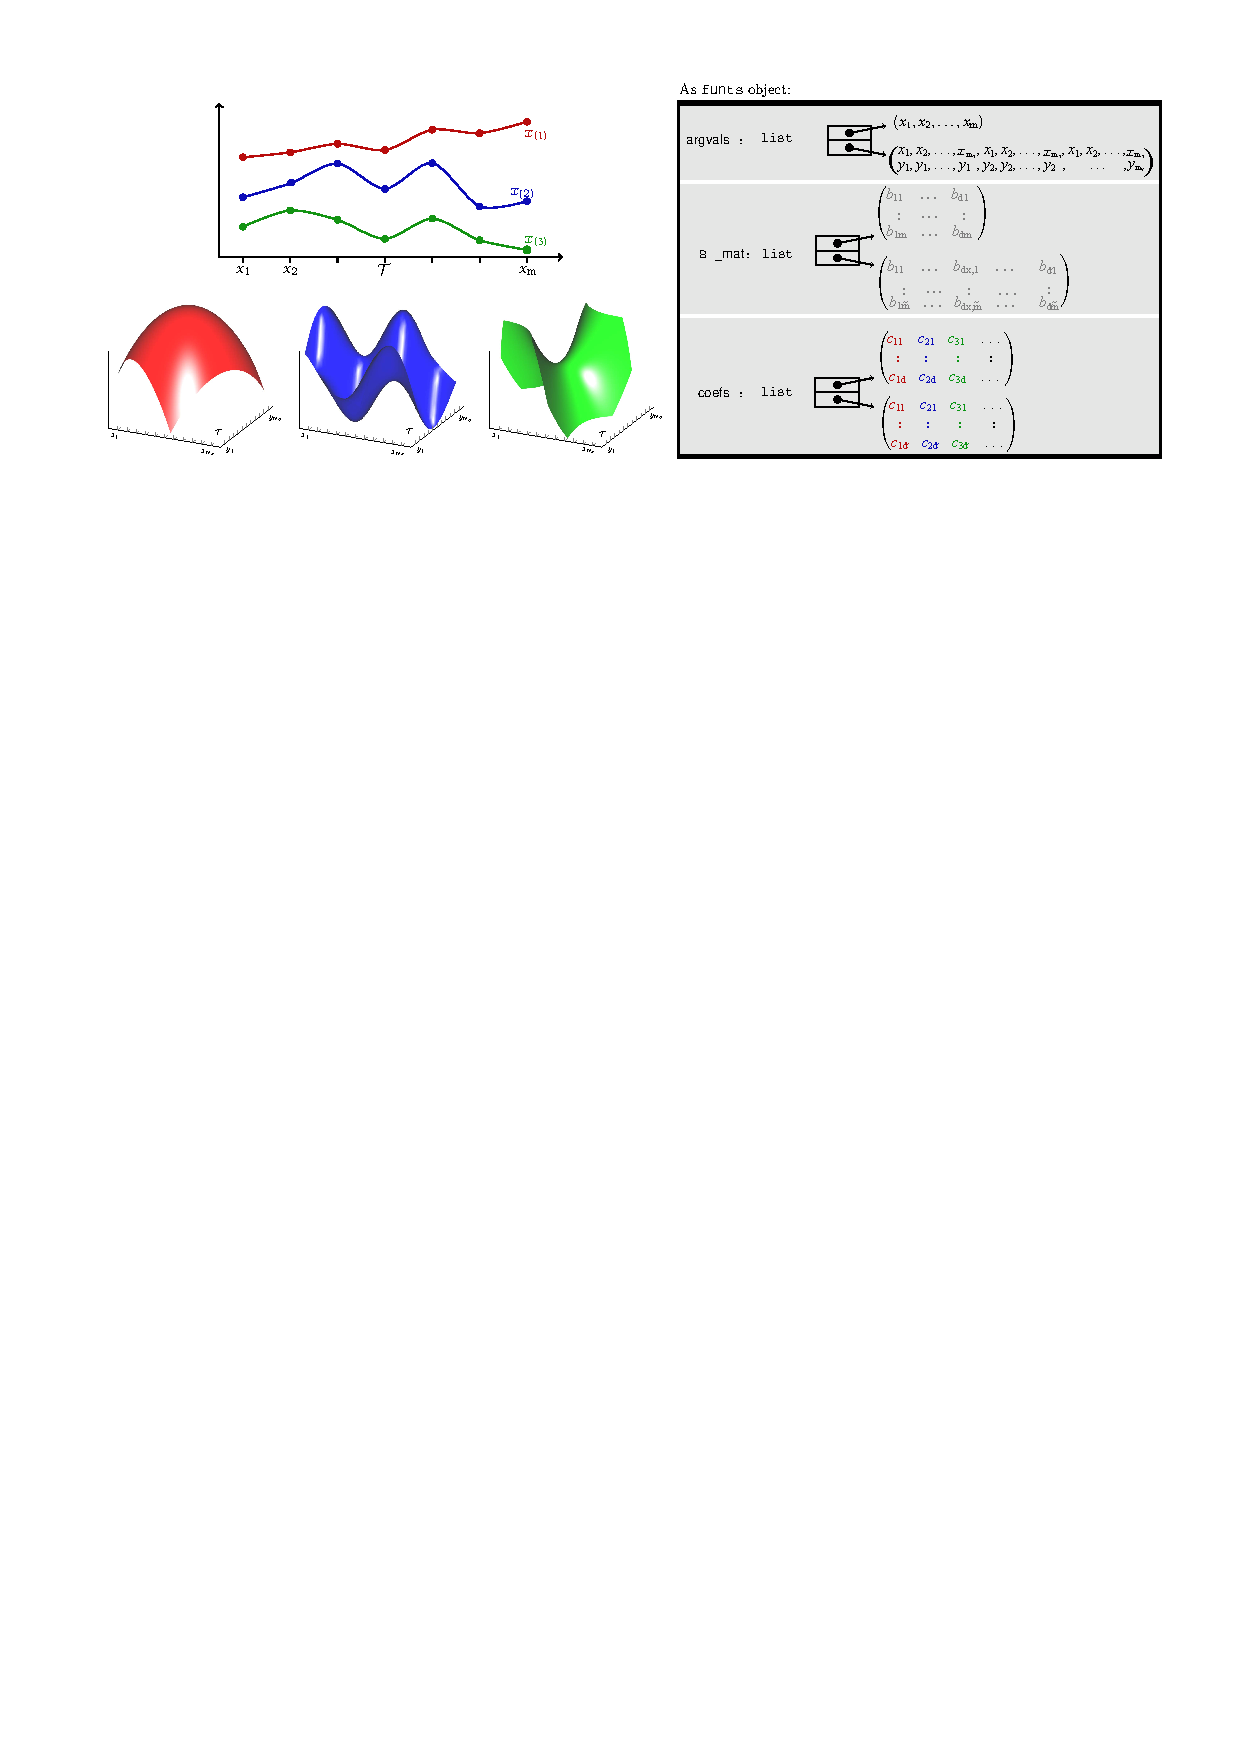
\includegraphics[page=1,width=0.9\textwidth]{figures/fts.pdf}
	\caption{The main roadmap of \code{funts} objects.  }
	\label{fig:fts}
\end{figure}

The \code{funts} class provides essential functionalities for managing FTS objects, ensuring users have well-defined basic operations. It supports arithmetic operations like addition and multiplication, along with indexing methods. Additionally, three generic methods, \code{length($\cdot$)}, \code{print($\cdot$)}, and \code{plot($\cdot$)}, are available. The \code{eval.funts($\cdot$)} method allows users to evaluate a \code{funts} object on a specified grid. To determine if an object belongs to the \code{funts} class, the \code{is.funts($\cdot$)} method is provided. Converting objects from the \CRANpkg{fda} package's \code{fd} class or the \CRANpkg{rainbow} package's \code{fts} class to a \code{funts} object is made easy using the \code{as.funts($\cdot$)} function. The strength of \code{funts} objects lies in their powerful visualization capabilities within the field of FTS. Users can create two types of plots using the graphical commands \code{plot($\cdot$)} and \code{plotly\_funts($\cdot$)}. The \code{plot($\cdot$)} method utilizes base graphics objects to generate FTS plots. On the other hand, the \code{plotly\_funts($\cdot$)} function offers a versatile \CRANpkg{plotly} platform for visualizing FTS data, providing several plot types: \code{line}, \code{3Dline}, \code{3Dsurface}, and \code{heatmap}. These plots making it easier to detect trends or patterns within each curve's behavior over time. Furthermore, users can directly apply \code{plotly\_funts($\cdot$)} function to objects from the \code{fd}, \code{fds}, or \code{fts} classes in packages like \CRANpkg{rainbow}, \CRANpkg{fds}, \CRANpkg{ftsa}, or \CRANpkg{fda}, without the need for conversion to \code{funts} objects. Additionally, when converting objects from packages like \code{fds} or \code{fts}, the \code{xname} and \code{yname} arguments are automatically captured and used as the \code{xlab} and \code{zlab} arguments, ensuring that resulting plots are informative and intuitive.

To demonstrate the capabilities of the \CRANpkg{Rfssa} package for handling FTS, two 
illustrative examples are provided. The first example showcases the \code{Callcenter} 
dataset consisting of curves observed over a one-dimensional domain. In contrast, 
the second example involves a bivariate FTS dataset, which includes a sequence of 
two types of remote sensing images (two-dimensional functional data domain).
\subsubsection{Example: Creating \code{funts} objects for FTS}
The first example uses the raw \code{Callcenter} dataset which was discussed before. The 
\code{funts} object can be made and plotted using the following codes. The generated 
plots are shown in Figure \ref{fig:call_center}.
\begin{example}
# Load necessary libraries
require(Rfssa)
require(fda)

# Load Callcenter data
Call_data <- loadCallcenterData()

# Prepare the data
D <- matrix(sqrt(Call_data$calls)), nrow = 240)
bs1 <- create.bspline.basis(c(0, 23), 22)

# Create a 'funts' object 
Call_funts <- funts(D, bs1, start = as.Date("1999-1-1"),
	vnames = "Sqrt of Call Numbers",
	dnames = "Time (6 minutes aggregated)",
	tname = "Date")

xtlab <- list(c("00:00", "06:00", "12:00", "18:00", "24:00"))
xtloc <- list(c(1, 60, 120, 180, 240))

# Generate a line plot using Plotly
plotly_funts(Call_funts, main = "Call Center Data Line Plot",
	xticklabels = xtlab, xticklocs = xtloc)

# Generate a heatmap plot using Plotly
plotly_funts(Call_funts, type = "heatmap", main = "Call Center Data Heatmap",
	xticklabels = xtlab, xticklocs = xtloc)

# Generate a 3D line plot using Plotly
plotly_funts(Call_funts, type = "3Dline", main = "Call Center Data 3Dline plot",
	xticklabels = xtlab, xticklocs = xtloc
)

# Generate a 3D surface plot using Plotly
plotly_funts(Call_funts, type = "3Dsurface", main = "Call Center Data 3Dsurface plot",
	xticklabels = xtlab, xticklocs = xtloc
)
\end{example}

\begin{figure}[ht!]
	\centering
	\begin{subfigure}[b]{0.4\textwidth}
		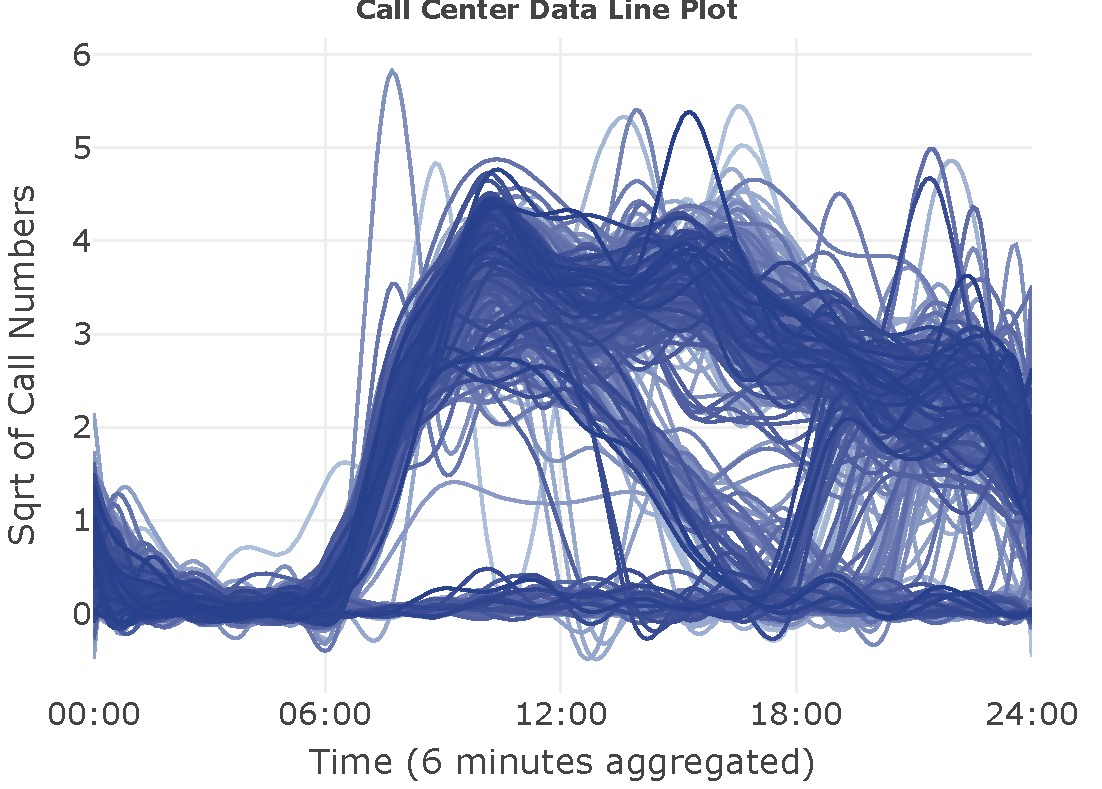
\includegraphics[page=1,width=\textwidth]{figures/call.pdf}
		\caption{The type of  \code{"line"}}
	\end{subfigure}
\hspace{.5in}	
	\begin{subfigure}[b]{0.4\textwidth}
		\includegraphics[page=2,width=\textwidth]{figures/call.pdf}
		\caption{The type of \code{"heatmap"}}
	\end{subfigure}	
	\begin{subfigure}[b]{0.49\textwidth}
\vspace{.2in}	
		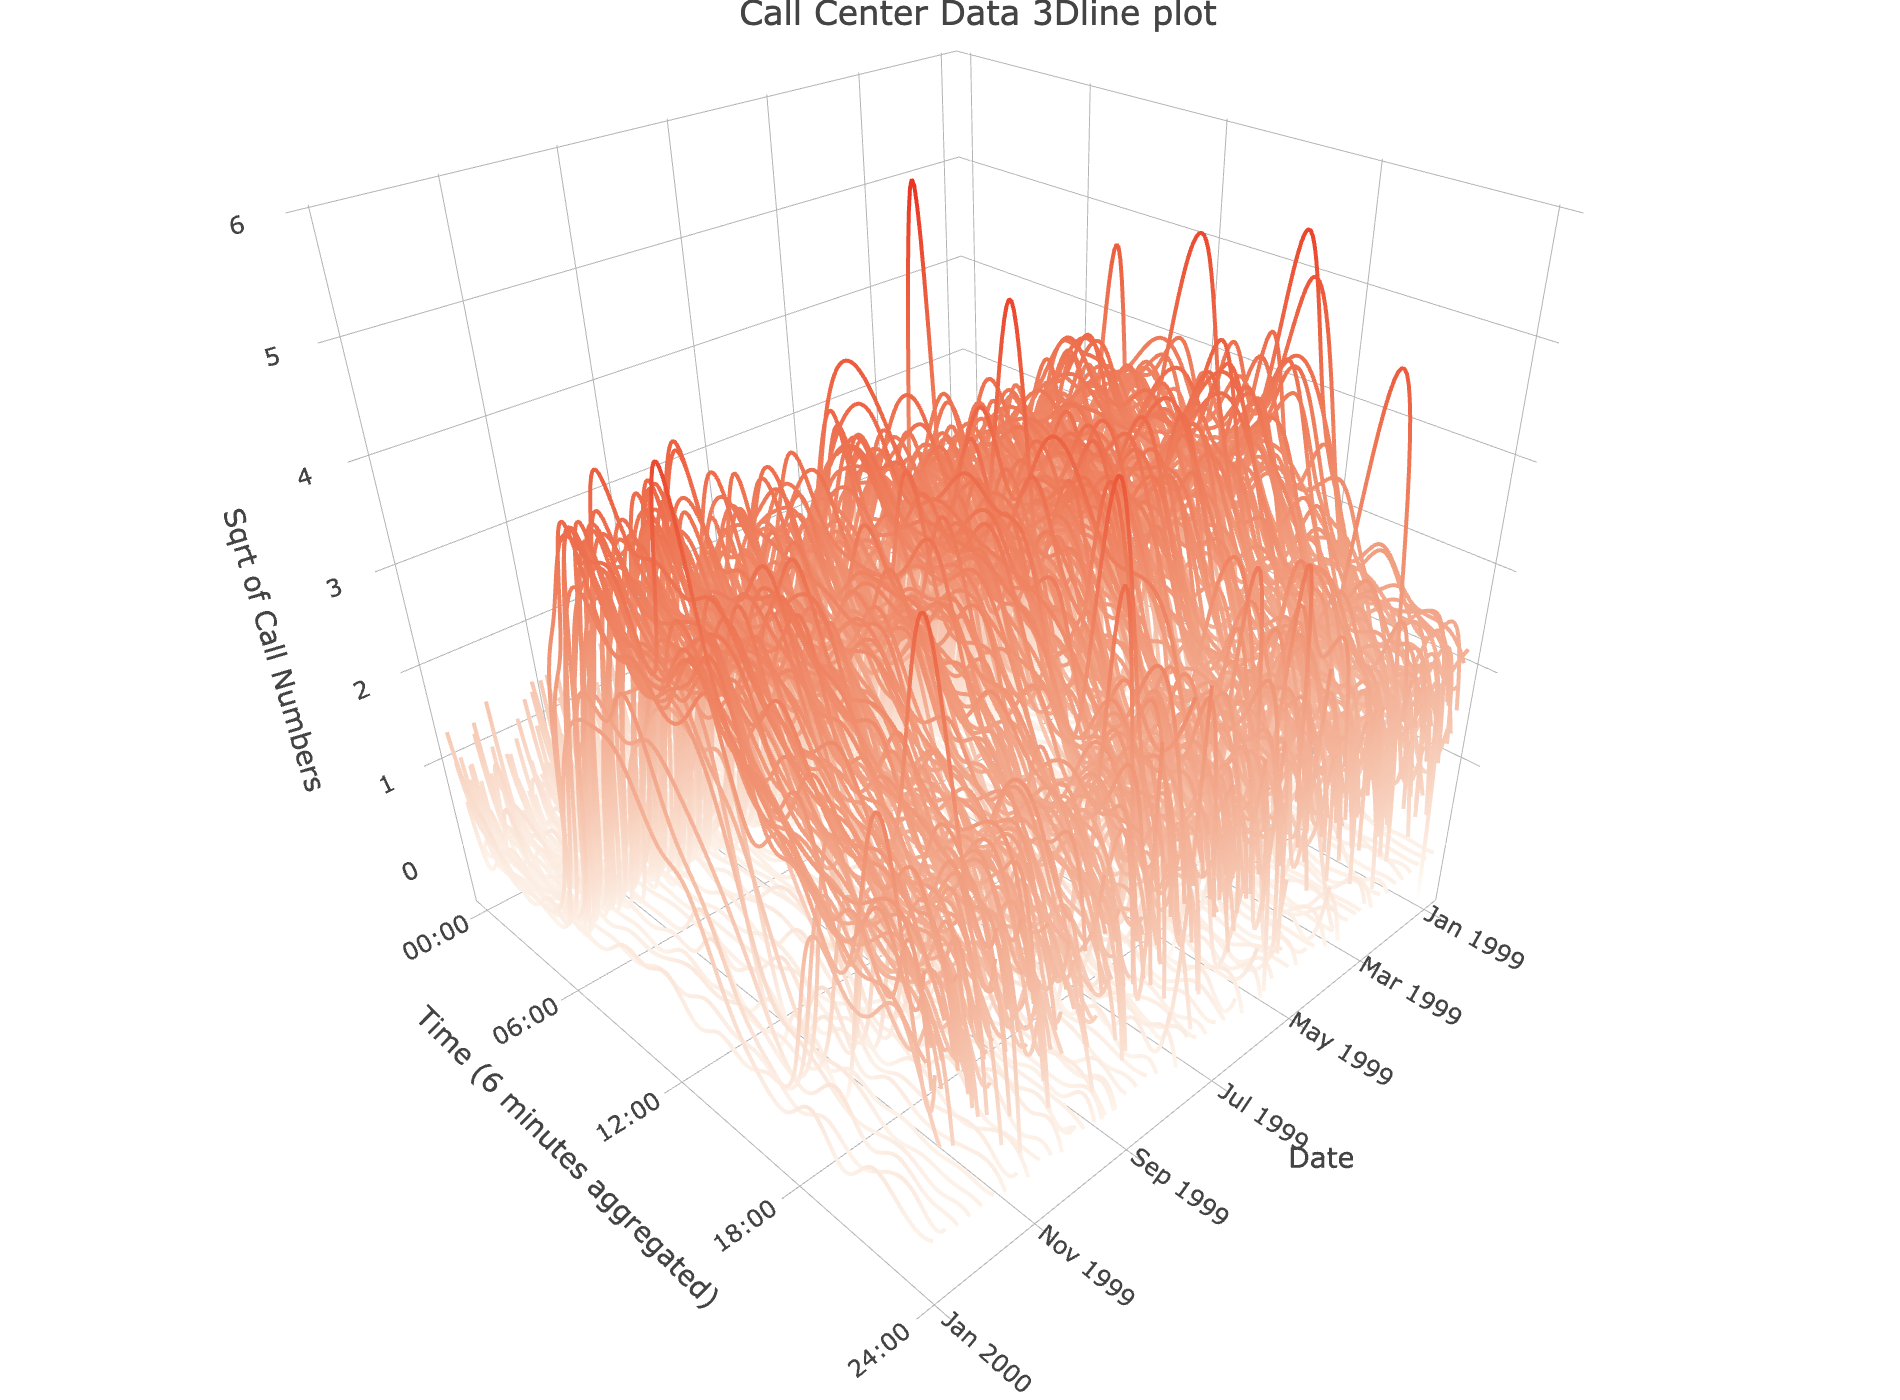
\includegraphics[width=\textwidth]{figures/3Dline.png}
		\caption{The type of \code{"3Dline"}}
	\end{subfigure}
	\begin{subfigure}[b]{0.49\textwidth}
		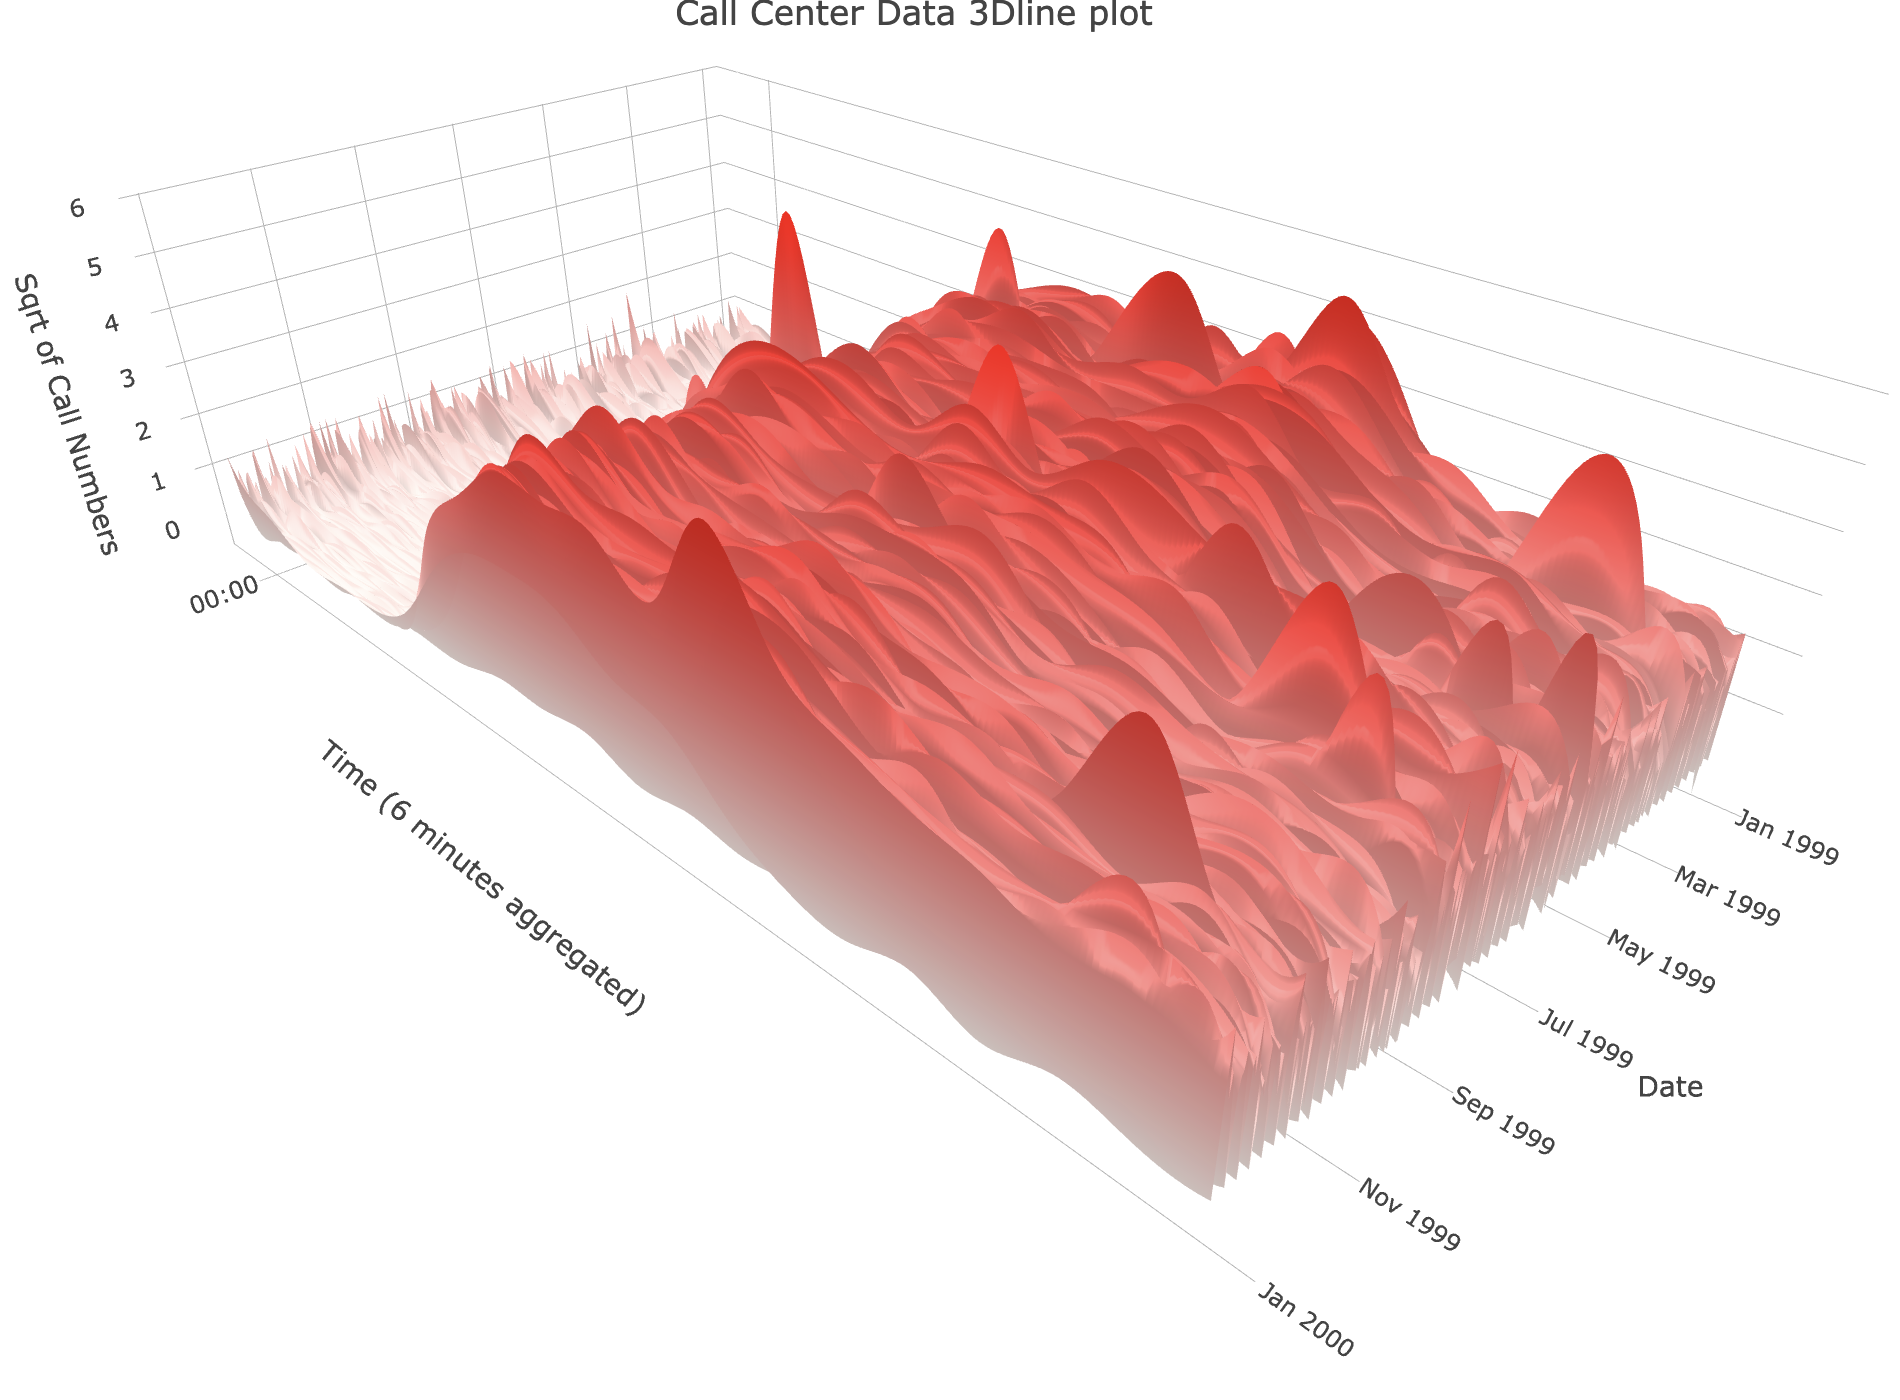
\includegraphics[width=\textwidth]{figures/3Dsurface.png}
		\caption{The type of \code{"3Dsurface"}}
	\end{subfigure}
	\caption{The plot types of the generated plots by \code{potly\_funts($\cdot$)}}
	\label{fig:call_center}
\end{figure}

As one can be see from Figure \ref{fig:call_center}(A), the overlapping line plot is 
a common way to view FTS data observed over a one-dimensional domain, where the 
curves that are recorded on dates closer to the start of 1999 are given in light 
blue while functions obtained on later dates are plotted in a darker blue. The 
heatmap plot in Figure \ref{fig:call_center}(B) is a newer technique used to 
visualize FTS data observed over a one-dimensional domain, allowing the user to see 
the evolution of the FTS over time as opposed to relying on different colorings of 
the curves to specify date. Such one-dimensional FTS can also be represented in a 
interactive 3D view. To obtain such plots the user simply needs to specify 
\code{type="3Dsurface"} or \code{type="3Dline"}.

\subsubsection{Example: Creating \code{funts} objects for MFTS}
The second example considered two collection of images where each image is drawn from a region southeast of the city of Jambi, Indonesia located between latitudes of $1.666792^{\circ}$ S - $1.598042^{\circ}$ S and longitudes of $103.608963^{\circ}$ E - $103.677742^{\circ}$ E. The images were recorded using the MODerate Resolution Imaging Spectroradiometer (MODIS) Terra satellite with a resolution of 250 meters every 16 days starting from February 18, 2000 and ending July 28, 2019. The output of each image is the normalized difference vegetation index (NDVI) which is used to quantify how much vegetation is present and enhanced vegetation index (EVI). The NDVI values closer to one being indicative of more vegetation and values closer to zero indicate less vegetation \citep[see][for more details]{haghbin2021}. The following code can be used to load the data, define a \code{funts} object for a MFTS, slice the \code{funts} object to select a specific variable (here NDVI),  and plot the smoothed images over time in an animation, that a snapshot is given in Figure \ref{fig:ndvi_image}. 

\begin{figure}[b!]
	\centering
	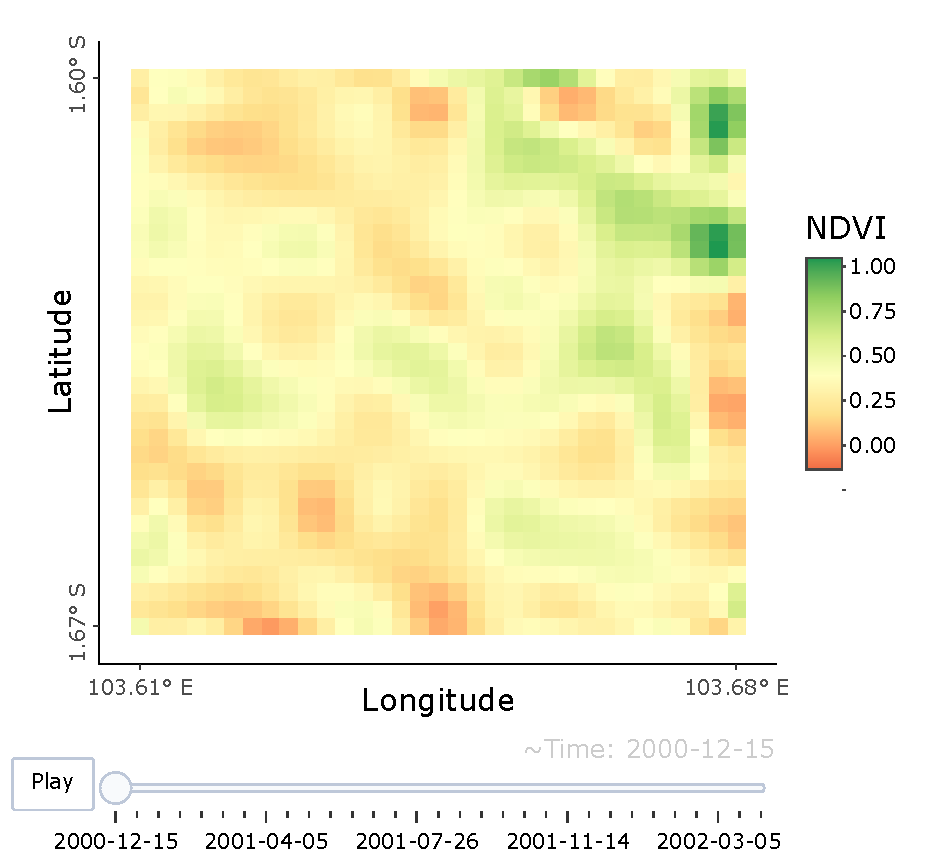
\includegraphics[width=.67\textwidth]{figures/ndvi.pdf}
	\caption{An NDVI snapshot from the city of Jambi, Indonesia.}
	\label{fig:ndvi_image}
\end{figure}

\begin{example}
# Load the Jambi dataset
Jambi <- loadJambiData()

# Extract NDVI and EVI array data 
NDVI <- Jambi$NDVI
EVI <- (Jambi$EVI)

# Create a list containing NDVI and EVI array data
Jambi_Data <- list(NDVI, EVI)

# Create a multivariate B-spline basis
require(fda)
bs2 <- create.bspline.basis(c(0, 1), 13)
bs2d <- list(bs2, bs2)
bsmv <- list(bs2d, bs2d)

# Create a funts object
Y_J <- funts(X = Jambi_Data,
	basisobj = bsmv,
	start = as.Date("2000-02-18"), end = as.Date("2019-07-28"),
	vnames = c("NDVI", "EVI"), tname = "Date",
	dnames = list(c("Latitude", "Longitude"), c("Latitude", "Longitude")))

# Create a Plotly-based visualization of the NDVI Image
plotly_funts(Y_J[, 1],
	main = "NDVI Image (Jambi)",
	xticklabels = list(c("103.61\u00B0 E", "103.68\u00B0 E")),
	yticklabels = list(c("1.67\u00B0 S", "1.60\u00B0 S")),
	xticklocs = list(c(0, 1)),
	yticklocs = list(c(0, 1)),
	color_palette = "RdYlGn")
\end{example}



\subsection{The \code{fssa} Class}\label{subsec:fssa}
 Once the \code{funts} object is created and $L$ is chosen, one can apply the \code{fssa($\cdot$)} constructor to obtain an \code{S3} object of class \code{fssa} that contains our singular values, left singular functions, and right singular vectors. %The  \code{type} argumet specifies the type of FSSA to perform, \code{type="ufssa"} to perform univariate FSSA (default for FTS) and \code{type="mfssa"} to perform MFSSA (default for MFTS). 
 An object of class \code{fssa}  is a list of right singular functions, which is packed in an object of class \code{funts} and the following components:
  \begin{itemize}
      \item[-] \code{values:} A numeric vector of singular values.
      \item[-] \code{L:} The specified window length.
  \item[-] \code{N:} The length of the functional time series. 
  \item[-] \code{Y:} The original \code{funts} object. 
  \end{itemize}

The generic \code{plot($\cdot$)} is developed for the \code{fssa} class to help the user make decisions on how to do the grouping stage of FSSA/MFSSA. This method, provides a complete set of visualization tools for the user to check the quality of the decomposition stage.  These SSA-type plots encompass various types, each providing unique insights into the data:
\begin{itemize}
	\item[-] \textbf{\code{"values"}}: Plots the singular values (default).
	\item[-] \textbf{\code{"paired"}}: Visualizes pairs of right singular vectors, which is particularly useful for detecting periodic components.
	\item[-] \textbf{\code{"wcor"}}: Generates a plot of the W-correlation matrix for the reconstructed objects.
	\item[-] \textbf{\code{"vectors"}}: Displays the right singular vectors, aiding in the detection of period length.
	\item[-] \textbf{\code{"lcurves"}}: Showcases the left singular functions, assisting in period length detection.
	\item[-] \textbf{\code{"lheats"}}: Heatmap plots of left singular functions are available, designed for \code{{funts}} variables observed over one or two-dimensional domains. These plots are valuable for identifying meaningful patterns.
	\item[-] \textbf{\code{"periodogram"}}: Periodogram plots of the right singular vectors can be generated, which help detect the frequencies of oscillations in functional data.
\end{itemize}
While efforts have been made to align these plots in \CRANpkg{Rfsaa} with the non-functional versions available in the \CRANpkg{Rsaa} package, there are some fundamental differences. Notably, \code{"lheats"} and \code{"lcurves"}  are novel plot types introduced in the \CRANpkg{Rfssa} package for functional data. Additionally, \code{"paired"} and \code{"vectors"}  types are developed based on the right singular vectors. All these plot types utilize the \CRANpkg{lattice} graphics engine. The following example codes generate these plots for the \code{Callcenter} dataset.

\subsubsection{Example: performing decomposition stage of FSSA}
In the rest of the paper, we will use  the pre-generated \code{funts} class object datasets such as 
\code{Callcenter} which are included within the package. These ready-to-use datasets serve as practical 
examples and templates, allowing users to test the FSSA procedure without the need 
to start from scratch with data preprocessing.
As mentioned previously, our approach involves performing FSSA with a lag window of 
$L=28$. We then generate a variety of SSA-type plots, as illustrated in Figure 
\ref{fig:call_decomp}, using the following code:
\begin{example}
# Load the Callcenter dataset
data("Callcenter")

# Perform FSSA:
fssa_results <- fssa(Callcenter, L = 28)

# FSSA plots:
plot(fssa_results, d = 9, type = "lcurves", 
	main = "(A) Left Singular Functions (within days)")
plot(fssa_results, d = 9, type = "lheats",
	main = "(B) Left Singular Functions (between days)")
plot(fssa_results, d = 13, main = "(C) Singular Values")
plot(fssa_results, d = 9, type = "vectors",
	main = "(D) Right Singular Vectors")
plot(fssa_results, d = 10, type = "paired",
	main = "(E) Paired Plots of Right Singular Vectors")
plot(fssa_results, d = 9, type = "wcor",
	main = "(F) W-Correlation Matrix")
\end{example}

\begin{figure}[t!]
	\centering
	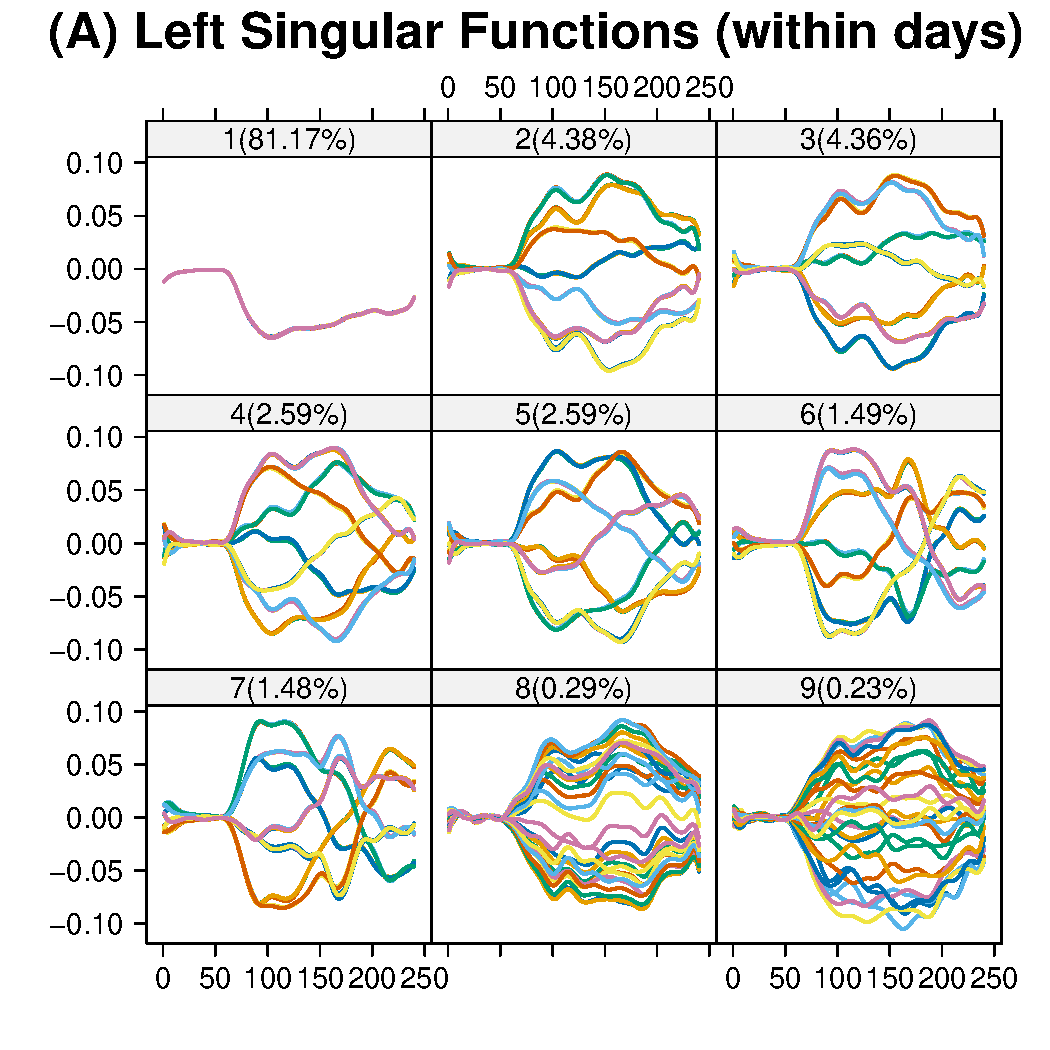
\includegraphics[page=1,width=.33\textwidth]{figures/fssa_call.pdf}
	\includegraphics[page=2,width=.33\textwidth]{figures/fssa_call.pdf}
	\includegraphics[page=3,width=.32\textwidth]{figures/fssa_call.pdf}
	\includegraphics[page=4,width=.33\textwidth]{figures/fssa_call.pdf}
	\includegraphics[page=5,width=.33\textwidth]{figures/fssa_call.pdf}
	\includegraphics[page=6,width=.32\textwidth]{figures/fssa_call.pdf}
	\caption{(A): Line plot of the left singular functions, used to identify 
	periodic and trend components; (B): Heatmap of the left singular functions; (C): 
	Scree plot of the singular values often used for grouping; (D): Right singular 
	vectors, used to identify periodic and trend components; (E): Paired plots of 
	the right singular vectors, used for grouping and identifying periodicity in the 
	FTS; (F): Weighted correlation (W-correlation) matrix used for grouping.}
	\label{fig:call_decomp}
\end{figure}

The W-correlation matrix in Figure \ref{fig:call_decomp}(F) is built by measuring 
the correlation between FTS that are reconstructed using the grouping of indices by 
setting $m=r$ (see the discussion on grouping in section 2). We also have that 
Figure \ref{fig:call_decomp}(E) is a plot of successive right singular vectors 
against one another. Using Figure \ref{fig:call_decomp}(C, E-F) we identify four 
groups in the \code{Callcenter} data such that $I_{1}=\{1\}$, $I_{2} = \{2,3\}$, 
$I_{3}=\{4,5\}$, and $I_{4}=\{6,7\}$.
Specifically, as discussed in \cite{golyandina2001}, periodic components in FTS typically exhibit a rank of 2, consisting of pairs of harmonic elementary components (sine and cosine functions with the same frequency). To identify these pairs, we can examine pairwise scatterplots of the right singular vectors, as illustrated in Figure \ref{fig:call_decomp}(E). In such scatterplots, components with identical frequencies, amplitudes, and phases form points that lie along a circular path. Additionally, the number of vertices in the resulting regular T-vertex polygon corresponds to the periodicity of the component. In Figure \ref{fig:call_decomp}(E), subplots 2 vs. 3, 4 vs. 5, and 6 vs. 7 reveal harmonic factors with frequencies of $1/7$, $8/14$, and $4/7$, respectively. For a more detailed exploration of extracting meaningful components from the extracted signal, additional references in the SSA literature, such as \cite{golyandina2013}, can be consulted.
In addition, using Figure 
\ref{fig:call_decomp}(A-B, D-E), we see clear weekly periodic patterns captured in 
the decomposition, for example the seven distinct curves found in various subplots 
of Figure \ref{fig:call_decomp}(A) and the seven corners seen in subplot 2 vs. 3 of 
Figure \ref{fig:call_decomp}(E).
For interested readers we provide further results for the decomposition stage and the \code{fssa} object in the GitHub repository of the \CRANpkg{Rfssa} package (\url{https://github.com/haghbinh/Rfssa}).


\section{Reconstruction and forecasting}
After obtaining an object of class \code{fssa}, the user may then choose to perform reconstruction using the \code{freconstruct($\cdot$)} function or perform forecasting using \code{fforecast($\cdot$)}. The reconstruction and forecasting functions both return a list of \code{funts} objects with length $m$ (number of groups). We note that even though it is common to perform forecasting using a combination of groups that best reconstructs the original signal, the user may try to forecast using several different combinations of groups.

\subsection{Reconstruction}
We start by reconstructing the \code{Callcenter} data using the grouping suggested 
from the FSSA decomposition. The following code implements the reconstruction 
methodology and gives the plots of the reconstruction in Figure 
\ref{fig:recon_call}. 
\begin{example}
# Define groups and their labels
groups <- list(1, 2:3, 4:5, 6:7, 1:7)
group_labels <- c("(B) First Group",
	"(C) Second Group",
	"(D) Third Group",
	"(E) Fourth Group",
	"(F) Extracted Signal")

# Perform FSSA‌ reconstruction
reconstructed_data  <- freconstruct(fssa_results, groups)

# Create and visualize plots
for (i in 1:length(groups)) {
  print(plotly_funts(reconstructed_data[[i]], main = group_labels[i], 
  		xticklocs = xtlab, xticklabels = xtloc))
}
\end{example}
One may observe the mean behavior (from group $I_1$) in Figure \ref{fig:recon_call}(C), and the weekly behaviors (from groups $I_2, I_3$ and $I_4$) in Figure \ref{fig:recon_call}(D-F). Note that the weekly trajectories are more well-separated in $I_4$ as opposed to the groups $I_2$ and $I_3$. We consider the last group, $I_{\mathfrak{s}}=\{1,\cdots,7\}$, as the set of indices corresponding to the leading eigentriples, that capture more than $98\%$ of the variation in the signal, to reconstruct the original FTS in Figure \ref{fig:recon_call}(B).

\subsection{The \code{fforecast} Class}
As previously mentioned, in addition to performing reconstruction of the FTS, the package offers the capability to perform forecasting using an object of class \code{fssa}. The constructor for this class, i.e., the \code{fforecast($\cdot$)} function, accepts the following arguments:
\begin{itemize}
	\item \code{U}: An object of class \code{fssa} holding the decomposition.
	\item \code{groups}: A list of numeric vectors where each vector is used for reconstruction and forecasting.
	\item \code{len}: An integer representing the desired length of the forecasted FTS.
	\item \code{method}: A character string specifying the type of forecasting to perform, with options including:
	\begin{itemize}
		\item "recurrent" for FSSA R-forecasting.
		\item "vector" for FSSA V-forecasting.
	\end{itemize}
	\item \code{only.new}: A logical argument, when set to \code{TRUE}, returns only the forecasted FTS, otherwise the entire FTS is returned.
\end{itemize}
The \code{fforecast($\cdot$)} function returns an S3 class named \code{fforecast}, which has been introduced to encapsulate the output of the function. This class is designed to provide a more organized and intuitive structure for handling FTS data. The \code{fforecast} class includes the following attributes:
\begin{itemize}
	\item \code{original\_funts}: This attribute stores the original FTS object, allowing users to maintain a clear reference to the original data.
	\item \code{predicted\_time}: Stores the forecast time index.
	\item \code{groups}: Contains a list of numeric vectors, where each vector includes indices of elementary components of a group used for reconstruction and forecasting.
	\item \code{method}: A character string specifying the type of forecasting performed.
\end{itemize}
To streamline user interactions further, we have developed a \code{print($\cdot$)} method for the \code{fforecast} class, making it more convenient to view and assess forecasted FTS data. To illustrate these enhancements, consider the continuous of Callcenter data example in the following:
\begin{example}
# Perform FSSA R-forecasting
pr_R <- fforecast(U = fssa_results, groups = c(1:3), len = 14, method = "recurrent")
# Perform FSSA V-forecasting
pr_V <- fforecast(U = fssa_results, groups = list(1,1:7), len = 14, method = "vector",
	only.new = FALSE)
	
plot(pr_R, main = 'R-Forecast (only.new = TRUE)')
plot(pr_V, main = 'V-Forecast (only.new = FALSE)')
print(pr_V)

# FSSA Forecast (fforecast) class:
# Groups: List of 2
# : num 1
# : int [1:7] 1 2 3 4 5 6 7
# Prediction method:  vector
# Predicted series length:  14
# Predicted time:  Date[1:14], format: "2000-01-01" "2000-01-02" ...

# ---------The original series-----------
# Functional time series (funts) object:
# Number of variables:  1
# Lenght:  365
# Start:  10592
# End:  10956
# Time:  Date[1:365], format: "1999-01-01" "1999-01-02" "1999-01-03"  ...
\end{example}
The resulted figure are shown in the Figure \ref{fig:forecast}.
\begin{figure}[h!]
	\centering
	\begin{minipage}{0.4\textwidth}
		\centering
		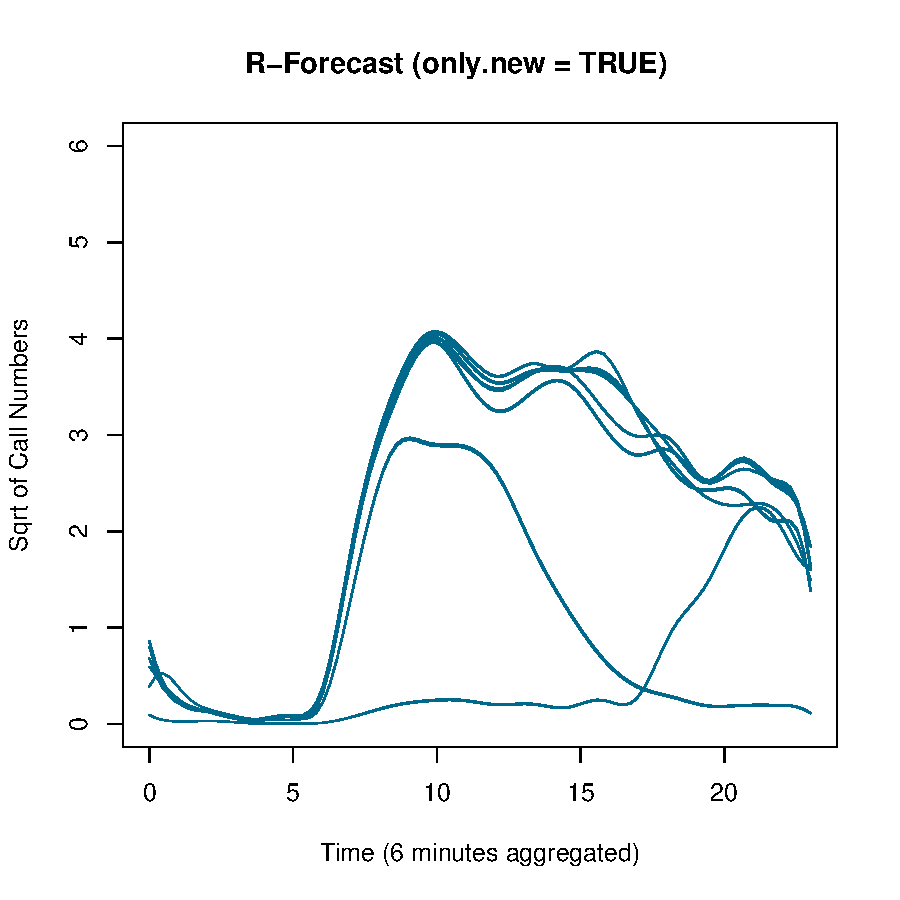
\includegraphics[width=\textwidth]{figures/Rfore.pdf}
	\end{minipage}%
	\begin{minipage}{0.4\textwidth}
		\centering
		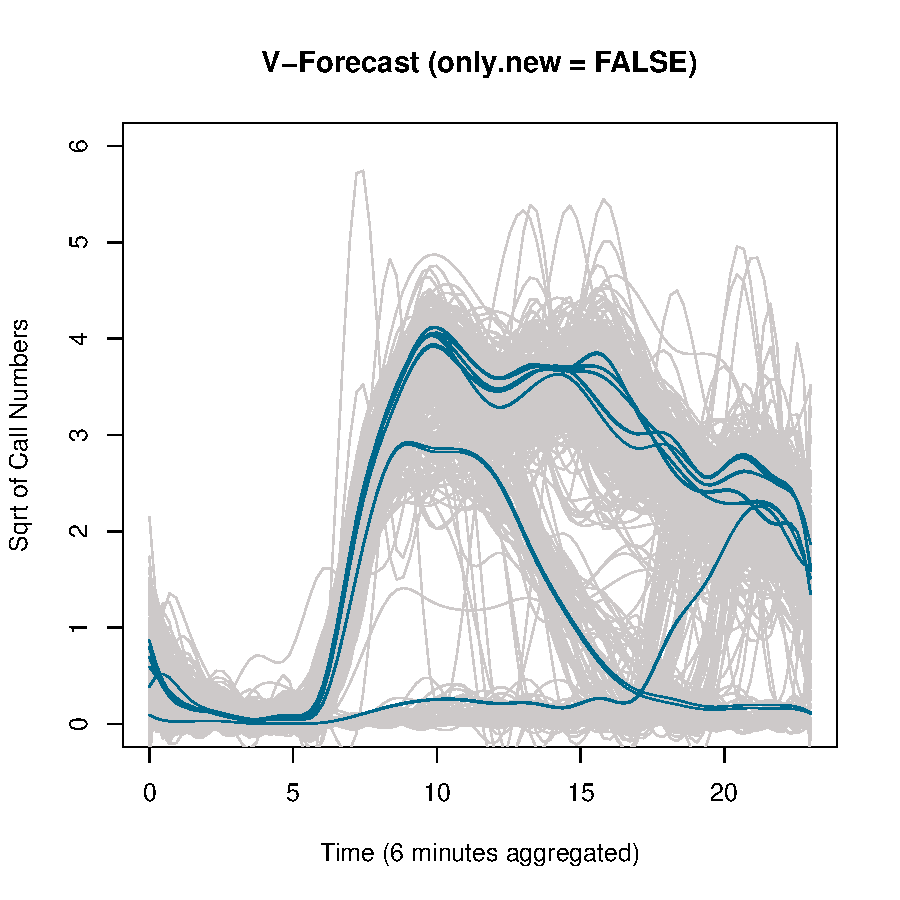
\includegraphics[width=\textwidth]{figures/Vfore.pdf}
	\end{minipage}
	\caption{\code{plot($\cdot$)} method of \code{fforecast} class.}
	\label{fig:forecast}
\end{figure}

The next example will forecast the \code{Callcenter} FTS one week into the future, based on the first $358$ days of the year, by leveraging the FSSA R-forecasting and V-forecasting methods as the results that had been given in the Figure \ref{fig:for_call}.
\begin{example}
# Define the data length
N <- Callcenter$N
U1 <- fssa(Callcenter[1:(N-7)], 28)

# Perform recurrent forecasting using FSSA
fore_R = fforecast(U1, groups = list(1:7), method = "recurrent", len = 7)[[1]]

# Perform vector forecasting using FSSA	
fore_V = fforecast(U1, groups = list(1:7), method = "vector", len = 7)[[1]]

# Extract the true call data
true_call <- Callcenter[(N-7+1):N]

# Define weekdays and colors
wd <- c('Sunday', 'Monday', 'Tuesday', 'Wednesday','Thursday', 'Friday', 'Saturday')
clrs <- c("black", "turquoise4", "darkorange")
argvals <- seq(0, 23, length.out = 100)
par(mfrow = c(1,7), mar = c(0.2, 0.2, 2, 0.2))

# Iterate over the days of the week
for(i in 1:7) {
	plot(true_call[i], col = clrs[1], ylim = c(0, 5.3),
		lty = 3, yaxt = "n", xaxt = "n", main = wd[i])
	plot(fore_R[i], col = clrs[2], lty = 2, add = TRUE)
	plot(fore_V[i], col = clrs[3], lty = 5, add = TRUE)
}
legend("top", c("Original", "R-forecasting", "V-forecasting"), col = clrs,
	lty = c(3, 2, 5))
\end{example}
 More information on these results may be found in the associated literature of \cite{haghbin2021} and \cite{trinka2023functional}.

\section{A shiny application}

The \CRANpkg{Rfssa} package contains shiny-apps for both FSSA and MFSSA methods. Those shiny-apps can be called using the \code{launchApp($\cdot$)} function, and also available in \url{http://sctc.mscs.mu.edu/fssa.htm} and \url{http://sctc.mscs.mu.edu/mfssa.htm}. Here we present the features of the MFSSA app, since the FSSA app would be a special case of that. MFSSA shiny-app was developed to visualize and extract the information related to MFTS in a non-parametric framework. The proposed shiny-app provides a friendly GUI for user to implement the \CRANpkg{Rfssa} functionalities and even compare the results with the non-functional version (\CRANpkg{Rssa}). 
 
Figure \ref{fig:shiny} provides a snapshot of the features available in MFSSA shiny-app. In the top of the side bar panel, user may specify the basis functions (B-spline or Fourier) and the associated degrees of freedom to represent the \code{funts} object. Those basis functions can be visualized in sub-panel \textsf{`Basis Functions'} under the main panel. The remaining inputs in the side bar will be used in other sub-panels. Specifically `Groups' is an input box for the third step of the MFSSA algorithm. Each group is specified via a vector (e.g. '\code{c(1,2,4)}' or '\code{1:3}') and separated from other groups with a comma (','). The slider `d' is used to specify the dimensions used in MFSSA (scree, W-correlation, paired, singular vectors \& functions, and periodogram plots). The check-box (a) `Demean' is used to subtract the mean to obtain mean-zero functions; (b) `Dbl Range' is used to extend the y-axis to cover all potential mirror functions (e.g. sometime FPCs may get multiply by a negative sign); and (c) `Univ. FSSA' to compare the MFSSA results with marginal FSSA ones respectively. The `Win.L.' slider specify the window lengths for the MSSA and the MFSSA. The `run M(F)SSA' button is used to run MSSA and MFSSA using the specified parameters for the given dataset. In general, for the side bar, the top inputs (above the red line) are mostly to describe the basis functions. The bottom inputs (below the red line) are used to specify SSA and FSSA parameters.

\begin{figure}[t]
	\centering
	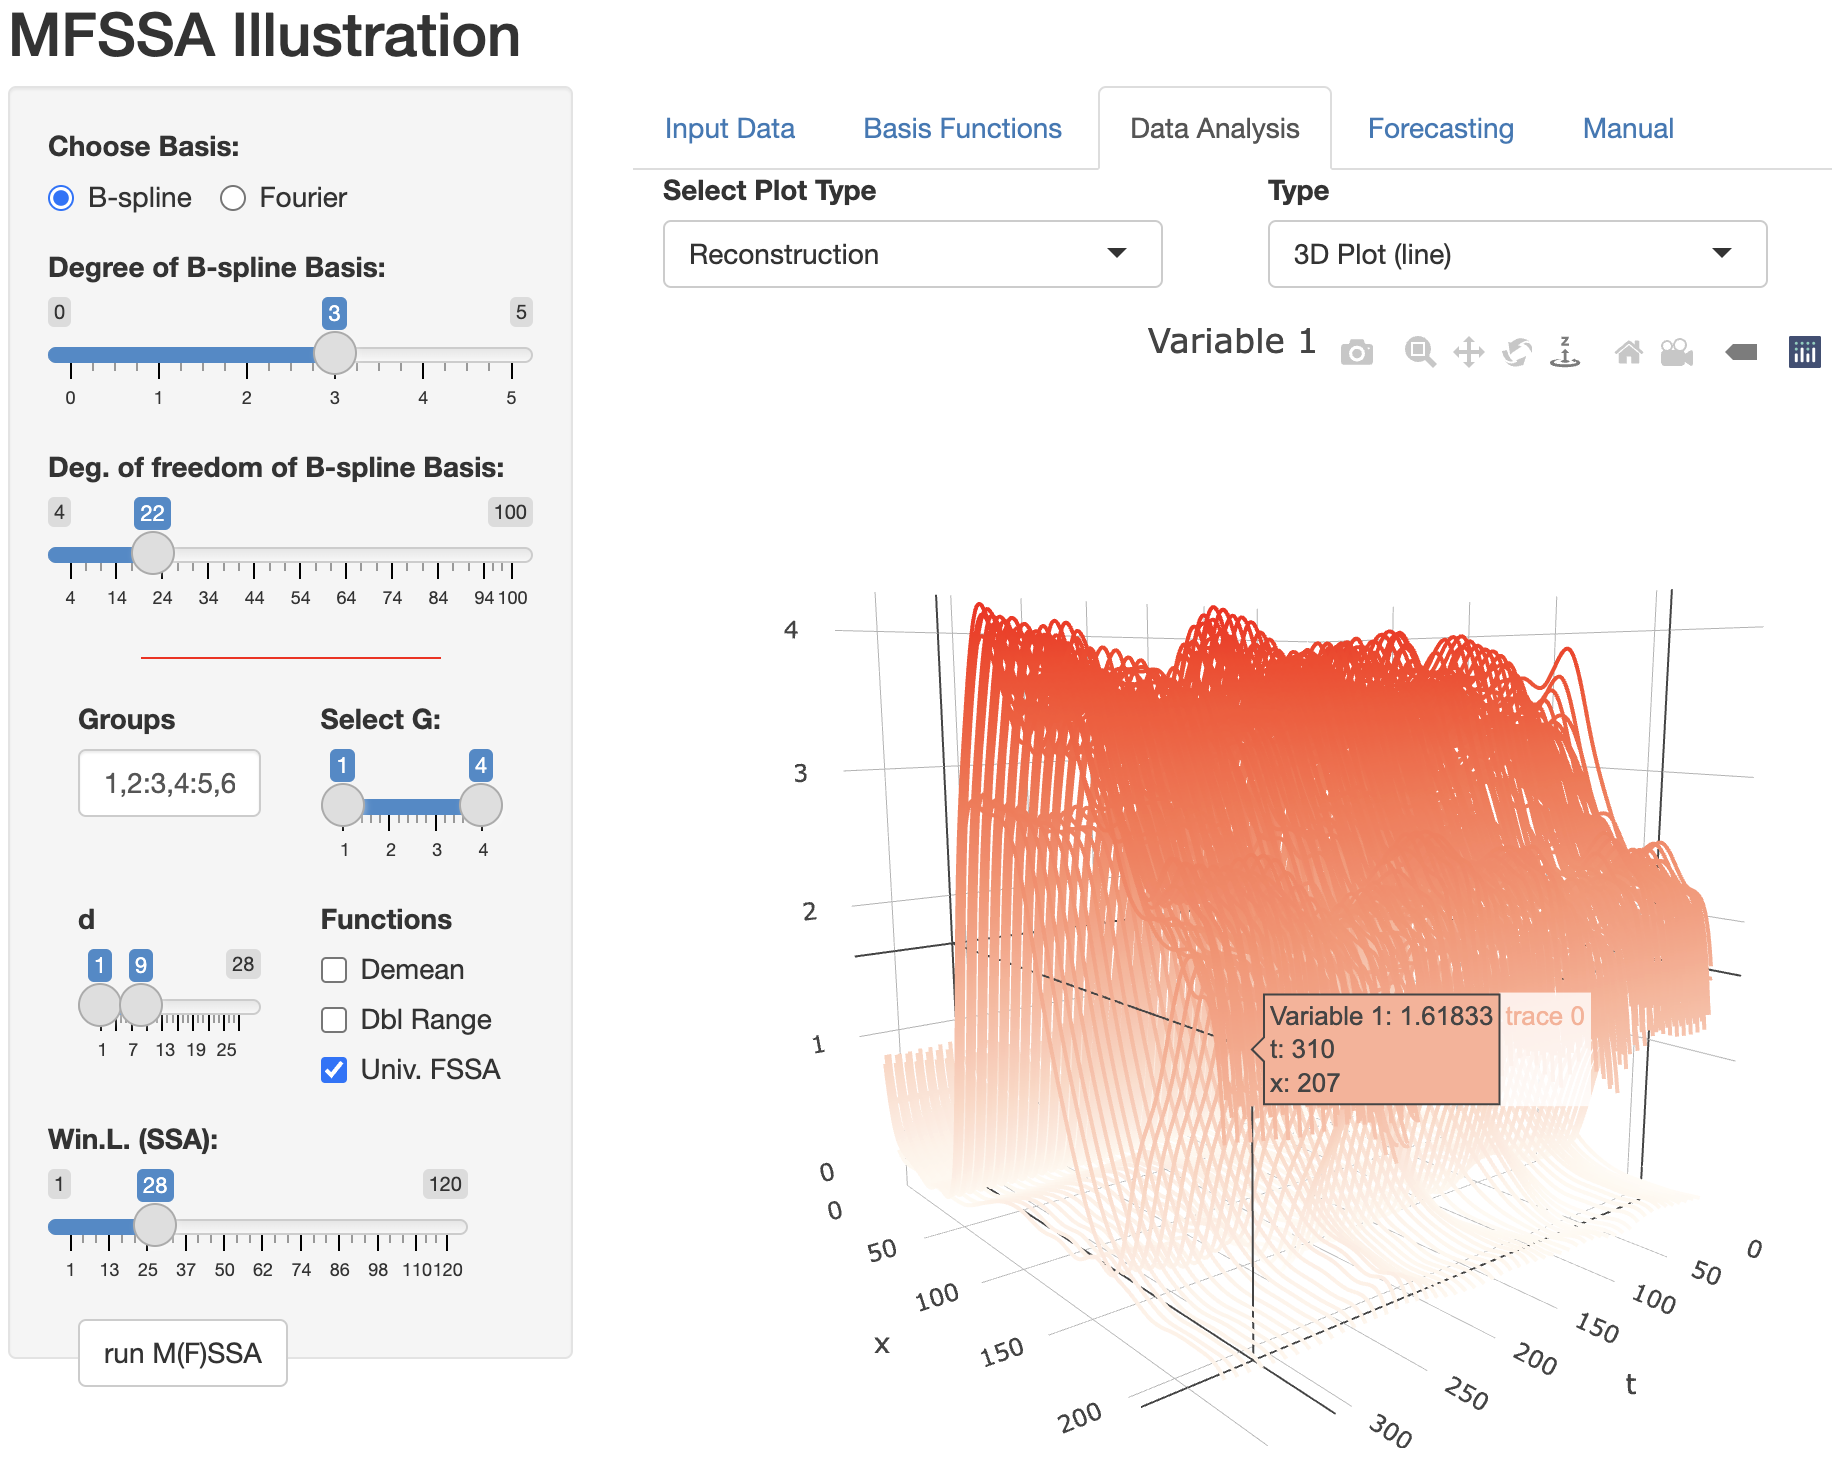
\includegraphics[width=\textwidth]{figures/shiny.png}
	\caption{Snapshot of the MFSSA shiny-app}
	\label{fig:shiny}
\end{figure}

The main panel includes five sub-panels. Here we briefly describe the features in each of these sub-panels:
\begin{itemize}
\item \textsf{`Input Data'}: In this sub-panel user can either (a) use the functional 
datasets available in the \CRANpkg{Rfssa} package (e.g, \code{Callcenter} data or remote 
sensing datasets); (b) simulate MFTS \citep[see][for details on simulation 
setup]{haghbin2021}; or (c) upload any arbitrary FTS matrix (where FTS are given in 
common grid-points and are represented in the columns of the data matrix) to provide 
the dataset and then analyze it.
\item \textsf{`Basis Functions'}: As described before we illustrate the basis functions selected by user in this sub-panel.
\item \textsf{`Data Analysis'}: In this sub-panel user can call variety of tools to
\begin{itemize}
\item visualize the MFTS.
\item obtain the optimal number of basis functions based on the GCV criteria.
\item select variety of outputs under MSSA and MFSSA, that includes scree plot, W-correlation plot, paired plots, singular vectors plots, periodogram plots, singular functions (heat or regular plots), and reconstruction of FTS using different type of plots (heat, regular, 3Dline and 3Dsurface). An example of the 3Dline reconstruction plot for the \code{Callcenter} data is given in Figure \ref{fig:shiny}.
\end{itemize}
\item \textsf{`Forecasting'}: This sub-panel would be accessible after user runs the MFSSA procedure, and it includes the functionalities of R-forecasting and V-forecasting algorithms.
\item \textsf{`Manual'}: This sub-panel provides a brief instruction manual to use the MFSSA shiny-app.
\end{itemize}

\section{Summary and conclusion}\label{sec:conclusion}
In summary, \textbf{Rfssa} is a pioneering package that brings the power of SSA to the realm of functional time series, offering novel techniques for decomposition, reconstruction, multivariate analysis, and functional forecasting. Its flexible data representation and functional context for SSA make it a valuable addition to the CRAN ecosystem, providing unique capabilities not readily available in other packages.

Notably, the package offers extensive capabilities for analyzing FTS/MFTS data, 
allowing joint analysis of smoothed curves and image data across different 
dimensional domains. The implementations of the methodologies in the 
package have been optimized for speed by leveraging the functionalities of 
\CRANpkg{RcppEigen} and \CRANpkg{RSpectra} R packages, along with custom 
\proglang{C++} code. By utilizing the \CRANpkg{Rfssa} package, researchers and 
practitioners can easily apply advanced FSSA-based techniques to their data, 
yielding informative results that can significantly enhance decision-making across 
various applied domains. The intuitive nature and computational efficiency of the 
package make it a valuable asset for the FTS analysis toolkit.

\section*{Acknowledgments}
The authors would like to express their sincere gratitude to the anonymous reviewers for their valuable feedback and constructive comments, which greatly contributed to the improvement of this work.
Additionally, we would like to acknowledge the significant contributions of Dr. S. Morteza Najibi during the development stages of the first version of the \CRANpkg{Rfssa} package. 


\bibliography{Haghbin_Rfssa}
\address{Hossein Haghbin\\
	Artificial Intelligence and Data Mining Research Group, ICT Research Institute \\
	Faculty of Intelligent Systems Engineering and Data Science, Persian Gulf University\\ Boushehr, Iran\\
	(ORCiD 0000-0001-8416-2354)\\
	\email{haghbin@pgu.ac.ir}}

\address{Jordan Trinka\\
  Department of Mathematical and Statistical Sciences, Marquette University,\\
  Wisconsin, USA\\
  (ORCiD 0000-0001-9118-5781)\\
  \email{jordantrinka4@hotmail.com}}


\address{Mehdi Maadooliat\\
  Department of Mathematical and Statistical Sciences, Marquette University,\\
  Wisconsin, USA\\
  (ORCiD: 0000-0002-5408-2676)\\
  \email{mehdi.maadooliat@mu.edu}}
